% Relazione - Cartella clinica passwordless
% Compilare con pdfLaTeX (default di Overleaf).
\documentclass[11pt,a4paper]{article}
\usepackage[utf8]{inputenc}
\usepackage[T1]{fontenc}
\usepackage[italian]{babel}
\usepackage{csquotes}
\usepackage{lmodern}
\usepackage[margin=2.5cm]{geometry}
\usepackage{microtype}
\usepackage{booktabs,array,graphicx,float}
\usepackage{listings,xcolor}
\usepackage{hyperref}
\usepackage{xurl}
\usepackage[backend=bibtex,style=numeric]{biblatex}
\addbibresource{riferimenti.bib}

\definecolor{accent}{HTML}{17695D}
\hypersetup{colorlinks=true,linkcolor=accent,urlcolor=accent,citecolor=accent}
\lstset{basicstyle=\ttfamily\small,columns=fullflexible,keepspaces=true,breaklines=true,frame=single,rulecolor=\color{gray!50},keywordstyle=\color{accent}\bfseries,commentstyle=\color{gray},showstringspaces=false,literate={à}{{\`a}}1 {è}{{\`e}}1 {é}{{\'e}}1 {ì}{{\`i}}1 {ò}{{\`o}}1 {ù}{{\`u}}1 {È}{{\`E}}1}
\lstdefinelanguage{Solidity}{keywords={contract,function,public,private,external,internal,view,pure,returns,require,emit,event,mapping,struct,modifier,address,uint256,bool,bytes32,string,memory,storage,if,else,for,return,import,pragma,constructor,enum,error,revert,is,immutable,constant,indexed,override,onlyRole,onlyOwner,whenNotPaused,uint64,uint8,uint48,delete},comment=[l]{//},morecomment=[s]{/*}{*/},morestring=[b]"}
\lstdefinelanguage{TypeScript}{keywords={const,let,var,function,return,if,else,for,of,in,await,async,new,class,interface,type,export,import,from,as,implements,private,readonly,static,try,catch,throw,true,false,null,undefined,void,string,number,boolean,Promise},sensitive=true,comment=[l]{//},morecomment=[s]{/*}{*/},morestring=[b]",morestring=[b]',morestring=[b]`}

\title{Cartella clinica passwordless:\\ consenso, accesso e audit con FIDO2, blockchain e prove a conoscenza zero}
\author{Raffaele \\ \small Laurea magistrale in Informatica, curriculum Sicurezza Informatica \\ \small Università degli Studi di Salerno}
\date{Corso di Sicurezza dei Dati \,---\, A.A. 2026/27 \\ \small Bozza v0.2}

\begin{document}
\maketitle
\begin{abstract}
% Da scrivere alla fine: problema, soluzione proposta, risultati principali (5-8 righe).
\end{abstract}
\tableofcontents
\newpage

\section{Introduzione}\label{sec:introduzione}

\subsection{Contesto e motivazione}
I dati sanitari sono una \emph{categoria particolare} di dati personali (art.~9 GDPR\cite{gdpr}): la loro diffusione può causare discriminazioni e danni difficili da rimediare. Eppure l'accesso a una cartella clinica elettronica si basa ancora spesso su password, che si possono rubare con il phishing o riusare da un servizio violato; il consenso del paziente è un documento che il sistema non verifica a ogni accesso; e il registro degli accessi è conservato e amministrato dallo stesso soggetto che dovrebbe essere controllato.

\subsection{Obiettivi}
Il progetto realizza il prototipo di una cartella clinica che affronta questi tre punti con strumenti visti nel corso:
\begin{itemize}
  \item \textbf{accesso senza password}: pazienti e medici si autenticano con una passkey FIDO2, resistente al phishing e al replay;
  \item \textbf{consenso verificabile e revocabile}: il paziente concede e revoca il consenso con il proprio wallet, per una finalità e fino a una scadenza, su uno smart contract che il backend consulta a ogni accesso;
  \item \textbf{audit non modificabile}: ogni accesso, concesso o negato, è registrato su blockchain prima che i dati vengano consegnati;
  \item \textbf{dati esposti al minimo}: sulla blockchain vanno solo pseudonimi e impronte, mentre referti e dettagli degli accessi restano fuori dalla catena, cifrati.
\end{itemize}
Per i dati che devono restare riservati per decenni, la cifratura e, dove l'autenticatore lo consente, le passkey usano anche algoritmi post-quantistici standardizzati dal NIST. I dati clinici usati sono esclusivamente sintetici.

\subsection{Contributi e struttura della relazione}
Il prototipo comprende un backend in TypeScript, un frontend React, due smart contract in Solidity e 191 test automatici; il codice è pubblico su GitHub. La relazione è organizzata così:
\begin{itemize}
  \item la sezione~\ref{sec:minacce} definisce requisiti e modello di minaccia;
  \item la sezione~\ref{sec:architettura} descrive l'architettura e cosa sta sulla catena;
  \item le sezioni~\ref{sec:fido2}, \ref{sec:blockchain} e~\ref{sec:dati} descrivono autenticazione FIDO2, consenso e audit su blockchain, protezione dei dati clinici;
  \item la sezione~\ref{sec:revisione} riporta la revisione di sicurezza del prototipo;
  \item le sezioni~\ref{sec:zkp} e~\ref{sec:fabric} discutono due alternative progettuali: le prove a conoscenza zero e una blockchain \emph{permissioned};
  \item la sezione~\ref{sec:valutazione} verifica i requisiti e misura costi e prestazioni; la sezione~\ref{sec:conclusioni} conclude.
\end{itemize}

\section{Requisiti e modello di minaccia}

\subsection{Attori e casi d'uso}
Il sistema gestisce l'accesso a cartelle cliniche sintetiche. Gli attori sono:

\begin{description}
  \item[Paziente] proprietario dei dati; concede e revoca il consenso all'accesso, separatamente per ogni finalità.
  \item[Medico] professionista abilitato; chiede l'accesso alla cartella di un paziente per una finalità dichiarata.
  \item[Medico di pronto soccorso] medico autorizzato anche all'accesso d'emergenza, senza consenso, quando il paziente non è in grado di darlo.
  \item[Struttura sanitaria] ente che identifica gli utenti e rilascia gli inviti, carica i referti, amministra i contratti e mantiene l'elenco dei medici abilitati (sezione~\ref{sec:zkp}).
  \item[Auditor] soggetto che verifica gli accessi, sul registro on-chain e su quello cifrato off-chain; per esempio il responsabile della protezione dei dati.
  \item[Avversario] chiunque tenti un accesso non autorizzato, dall'esterno o dall'interno (sezione~\ref{sec:minacce}).
\end{description}

I casi d'uso principali sono: registrazione e revoca di una passkey, accesso del medico, concessione e revoca del consenso, consultazione di una cartella, accesso d'emergenza, consultazione dell'audit.

\subsection{Requisiti funzionali}
\begin{table}[H]
\centering\small
\begin{tabular}{@{}l p{.78\textwidth}@{}}
\toprule
ID & Requisito\\
\midrule
RF1 & Registrazione e accesso degli utenti senza password, con credenziali FIDO2/WebAuthn.\\
RF2 & Il paziente può concedere il consenso a un medico per una specifica finalità (cura, ricerca, amministrazione), con scadenza, e revocarlo in qualsiasi momento.\\
RF3 & Un medico può leggere una cartella solo se è abilitato e ha un consenso valido per la finalità dichiarata.\\
RF4 & Ogni tentativo di accesso, riuscito o negato, lascia una traccia di audit non modificabile.\\
RF5 & Il medico dimostra di essere abilitato senza rivelare la propria identità alla blockchain (ZKP).\\
RF6 & I dati clinici sono cifrati a riposo e non compaiono mai sulla blockchain.\\
RF7 & Il paziente e l'auditor possono verificare lo storico degli accessi.\\
RF8 & In emergenza un medico autorizzato può accedere senza consenso, con motivazione obbligatoria e traccia separata nell'audit.\\
RF9 & Un utente può revocare una propria passkey (per esempio di un dispositivo perso) e chiudere tutte le proprie sessioni.\\
RF10 & Il medico che ha in cura il paziente può aggiungere alla cartella un referto firmato con la propria passkey.\\
\bottomrule
\end{tabular}
\caption{Requisiti funzionali.}
\end{table}

\subsection{Requisiti non funzionali}
\begin{table}[H]
\centering\small
\begin{tabular}{@{}l p{.78\textwidth}@{}}
\toprule
ID & Requisito\\
\midrule
RNF1 & Resistenza al phishing e al replay nell'autenticazione.\\
RNF2 & Riservatezza e integrità dei dati clinici (cifratura autenticata), anche contro un avversario dotato in futuro di un computer quantistico.\\
RNF3 & Integrità e non ripudio dell'audit.\\
RNF4 & Conformità ai principi del GDPR: limitazione della finalità, minimizzazione dei dati e possibilità di cancellazione dei dati personali.\\
RNF5 & Sicurezza degli smart contract rispetto alle vulnerabilità note (reentrancy, controllo degli accessi, ecc.).\\
RNF6 & Costi di gas contenuti per le operazioni più frequenti.\\
RNF7 & Comportamento sicuro in caso di guasto (\emph{fail-closed}): se l'audit non è disponibile, nessun dato viene consegnato.\\
\bottomrule
\end{tabular}
\caption{Requisiti non funzionali.}
\end{table}

\subsection{Assunzioni}
\begin{itemize}
  \item Gli autenticatori FIDO2 dei medici e dei pazienti sono dispositivi non compromessi.
  \item La blockchain è considerata corretta e disponibile: non si modellano attacchi al consenso della rete.
  \item Il backend è un componente semi-fidato: può sbagliare o essere compromesso, ma non può riscrivere l'audit né creare un consenso al posto del paziente.
  \item La procedura di identificazione con cui la struttura rilascia gli inviti è affidabile.
  \item Si usano esclusivamente dati clinici sintetici.
\end{itemize}

\subsection{Modello di minaccia}\label{sec:minacce}
Le minacce sono classificate con le categorie STRIDE (Spoofing, Tampering, Repudiation, Information disclosure, Denial of service, Elevation of privilege). Le righe da M13 in poi sono emerse dalla revisione di sicurezza descritta nella sezione~\ref{sec:revisione}.

\begin{table}[H]
\centering\footnotesize
\renewcommand{\arraystretch}{1.25}
\begin{tabular}{@{}l p{.22\textwidth} p{.36\textwidth} p{.2\textwidth}@{}}
\toprule
ID & Minaccia (STRIDE) & Contromisura & Verifica\\
\midrule
M1 & Furto o riuso di credenziali, phishing (S) & Passkey FIDO2 legate all'origine; nessuna password da rubare & Test, sez.~\ref{sec:fido2-test}\\
M2 & Replay di una risposta di autenticazione (S) & Challenge casuale a uso singolo con scadenza & Test, sez.~\ref{sec:fido2-test}\\
M3 & Clonazione dell'autenticatore (S) & Controllo atomico di signCount; revoca della credenziale & Test, sez.~\ref{sec:fido2-test}\\
M4 & Modifica o cancellazione dei log di audit (T, R) & Log su blockchain in sola aggiunta; dettagli off-chain legati all'impronta on-chain & Test, sez.~\ref{sec:test}\\
M5 & Medico che nega di aver letto una cartella (R) & Evento on-chain legato all'indirizzo del medico & Sez.~\ref{sec:blockchain}\\
M6 & Lettura non autorizzata di una cartella (I) & Consenso on-chain per finalità, ruolo verificato, cifratura dei referti & Test, sez.~\ref{sec:accesso} e~\ref{sec:dati}\\
M7 & Dati personali scritti sul ledger (I) & Sul ledger solo pseudonimi, impronte con nonce e prove; dati off-chain & Sez.~\ref{sec:architettura}; EDPB\cite{edpb-blockchain}\\
M8 & Vulnerabilità del contratto (T, E) & Pattern di sicurezza, librerie collaudate, test & Sez.~\ref{sec:blockchain}\\
M9 & Un account ottiene ruoli o consensi non suoi (E) & Controllo del chiamante nel contratto; mai \texttt{tx.origin} & Test, sez.~\ref{sec:test}\\
M10 & Indisponibilità del servizio (D) & Limite di frequenza per client e per utente; login non bloccabile da terzi & Test, sez.~\ref{sec:revisione}\\
M11 & Backend compromesso (T, I) & Non può scrivere consensi né riscrivere l'audit; un accesso concesso richiede un consenso valido sulla catena & Test, sez.~\ref{sec:accesso}\\
M12 & Registrazione di una passkey sull'account di un altro utente (S, E) & Invito monouso legato all'utente, o sessione dello stesso utente & Test, sez.~\ref{sec:fido2-autorizzazione}\\
M13 & Scoperta degli utenti registrati (I) & Opzioni di login identiche per ogni username & Test, sez.~\ref{sec:revisione}\\
M14 & Dettagli interni nei messaggi d'errore (I) & Gestore finale degli errori con messaggi generici & Test, sez.~\ref{sec:revisione}\\
M15 & Lettura diretta del database (I) & Referti e registro degli accessi cifrati; token e inviti solo come hash & Test, sez.~\ref{sec:dati}\\
M16 & Furto o perdita delle chiavi dell'archivio (I, D) & Chiavi cifrate con passphrase (Argon2id); backup a soglia 3 su 5 & Test, sez.~\ref{sec:chiavi}\\
M17 & Dispositivo perso o rubato (S) & Revoca della passkey e chiusura di tutte le sessioni; durata massima della sessione & Test, sez.~\ref{sec:fido2-revoca}\\
M18 & Furto della chiave che amministra i contratti (E) & Passaggio di consegne in due fasi con attesa; pausa con ruolo separato & Test, sez.~\ref{sec:test}\\
M19 & Abuso dell'accesso d'emergenza (E, R) & Ruolo dedicato, motivazione obbligatoria, evento separato; tentativi respinti registrati & Test, sez.~\ref{sec:accesso}\\
M20 & Correlazione dei metadati pubblici sulla catena (I) & Pseudonimi dedicati; mitigazione completa solo con rete permissioned & Rischio residuo, sez.~\ref{sec:revisione}\\
M21 & Referto alterato o attribuito a un altro medico; medico che nega di averlo scritto (T, R, S) & Firma con la passkey del medico sull'impronta del referto, verificata a ogni consegna & Test, sez.~\ref{sec:firma}\\
\bottomrule
\end{tabular}
\caption{Modello di minaccia.}
\end{table}

I rischi che restano dopo le contromisure sono raccolti nella sezione~\ref{sec:residui}.

\section{Architettura}\label{sec:architettura}

\subsection{Panoramica}
Il sistema è una DApp in cinque parti (tabella~\ref{tab:componenti}). Paziente e medico usano un'applicazione web, che dialoga con il backend per identità e dati clinici e direttamente con la blockchain, tramite il wallet del paziente, per concedere o revocare un consenso.

\begin{table}[H]
\centering\footnotesize
\renewcommand{\arraystretch}{1.2}
\begin{tabular}{@{}p{.17\textwidth}p{.27\textwidth}p{.38\textwidth}p{.1\textwidth}@{}}
\toprule
Componente & Tecnologia & Compito & Stato\\
\midrule
Frontend & React, Vite, WebAuthn del browser & Accesso con passkey, gestione delle proprie passkey e delle sessioni, consultazione delle cartelle e firma dei referti, concessione e revoca dei consensi con il wallet del paziente, registro degli accessi verificabile sulla catena & Completo\\
Backend & Node.js 24, TypeScript, Express 5, ethers 6 & Autenticazione FIDO2, sessioni, controllo degli accessi, cifratura e firma dei referti, scrittura dell'audit, registro per il paziente, cancellazione su richiesta & Completo\\
Database & MongoDB 8.0 & Utenti, credenziali FIDO2, sessioni, profili, referti cifrati, registro cifrato degli accessi & Completo\\
Custodia delle chiavi & AES-256-GCM, ML-KEM-768 + X25519, Argon2id, Shamir & Chiavi dell'archivio cifrate con passphrase, backup a soglia & Completo\\
Smart contract & Solidity 0.8, OpenZeppelin, Hardhat & Registro dei consensi per finalità, registro di audit con accessi d'emergenza, amministrazione con passaggio di consegne & Completo\\
\bottomrule
\end{tabular}
\caption{Componenti del sistema e stato del prototipo.}\label{tab:componenti}
\end{table}

Il backend è l'unico componente che vede i dati clinici in chiaro, e solo per servirli a un utente autorizzato, ma non è l'unica fonte di verità: non può concedere consensi al posto del paziente, perché il contratto accetta solo transazioni firmate dal paziente; non può registrare come autorizzato un accesso senza consenso, perché il registro di audit lo rifiuta; non può riscrivere gli accessi registrati, perché il registro è in sola aggiunta. Compromettere il backend non basta quindi a nascondere un accesso abusivo.

\subsection{Organizzazione secondo il pattern MVC}
Il codice segue il pattern Model-View-Controller, adattato alla presenza di due archivi, uno tradizionale e uno distribuito. Il \textbf{Model} conserva lo stato del sistema dietro tre interfacce:
\begin{itemize}
  \item \texttt{Store}, le operazioni sui dati off-chain, implementata da \texttt{MongoStore} nel server e da \texttt{MemoryStore} nei test;
  \item \texttt{Ledger}, la vista sulla blockchain (leggere un consenso, scrivere una voce di audit), implementata da \texttt{EthersLedger}, che parla con i contratti, e da \texttt{MemoryLedger}, che ne riproduce le regole nei test;
  \item \texttt{Vault}, che custodisce le chiavi dell'archivio e offre solo cifratura e decifratura, senza esporre le chiavi.
\end{itemize}
Sulla catena il Model sono gli smart contract.

La \textbf{View} è il frontend React, che non contiene regole di sicurezza: ogni decisione è presa dal backend o dai contratti. I \textbf{Controller} sono le funzioni del backend che validano la richiesta, applicano le regole (passkey, ruolo, consenso, sessione) e interrogano il Model; le rotte li collegano ai middleware comuni (sessione, limite di frequenza, intestazioni di sicurezza, gestione degli errori).

La separazione serve alla sicurezza: i vincoli importanti, come l'unicità di una credenziale o il consumo atomico di una challenge, stanno in un solo punto e non possono essere dimenticati in una rotta. Inoltre l'applicazione riceve il Model dall'esterno (\texttt{createApp(store, ledger, vault)}), quindi i test eseguono lo stesso codice dei controller che gira nel server.

\subsection{Cosa sta sulla blockchain e cosa no}
Sulla blockchain non compare alcun dato sanitario né alcun dato che identifichi direttamente una persona: solo indirizzi pseudonimi, finalità e scadenze dei consensi, esiti degli accessi e impronte crittografiche. Referti, dettagli degli accessi e credenziali restano fuori, cifrati e sotto il controllo della struttura.

Ciò che sta su un registro distribuito è replicato su tutti i nodi e non si cancella; per questo le linee guida dell'EDPB\cite{edpb-blockchain} chiedono di non scrivere dati personali sulla catena e di permettere la cancellazione fuori da essa. Le impronte sono calcolate su dettagli che contengono un valore casuale (\emph{nonce}), quindi non si ricostruiscono provando tutte le combinazioni di medico, paziente e finalità. Il paziente compare con un indirizzo dedicato ai soli consensi, il cui legame con la persona sta nel database e può essere cancellato (sezione~\ref{sec:cancellazione}). Restano visibili alcuni metadati, discussi tra i rischi residui (sezione~\ref{sec:residui}).

\subsection{Flusso di accesso a una cartella}\label{sec:flusso}
Un accesso del medico alla cartella di un paziente attraversa quattro controlli, nell'ordine:
\begin{enumerate}
  \item \textbf{autenticazione}: il medico accede con la propria passkey e ottiene una sessione (sezione~\ref{sec:fido2});
  \item \textbf{ruolo e consenso}: il backend verifica che chi chiede abbia il ruolo di medico, assegnato dalla struttura, e che il paziente gli abbia concesso, sul registro on-chain, un consenso ancora valido per la finalità dichiarata;
  \item \textbf{audit}: l'esito, concesso o negato, viene scritto sul registro di audit; se la scrittura non riesce, nulla viene consegnato;
  \item \textbf{consegna}: solo a questo punto i referti vengono decifrati in memoria e consegnati.
\end{enumerate}
Per le situazioni d'emergenza esiste un percorso separato, che salta il controllo del consenso ma lascia una traccia distinta nell'audit (sezione~\ref{sec:accesso}). Una prova di abilitazione a conoscenza zero, descritta come estensione nella sezione~\ref{sec:zkp}, si inserirebbe tra il primo e il secondo controllo.

\subsection{Ambiente e gestione delle dipendenze}
La versione di Node.js è fissata in \texttt{.nvmrc}, quelle delle librerie nei \texttt{package-lock.json}, quella del database in \texttt{docker-compose.yml}: i risultati sono riproducibili e un aggiornamento automatico non può introdurre una dipendenza compromessa. L'immagine del database è indicata con la versione esatta, la 8.0.38, e con la sua impronta (\emph{digest}), così Docker usa sempre esattamente quella immagine. La serie~8.0 è supportata dal produttore fino a ottobre 2029 e riceve correzioni di sicurezza\cite{mongodb-lifecycle}, mentre le serie intermedie hanno un supporto molto più breve. Le versioni~8.x non si avviano sui kernel Linux dalla 6.19 alla 7.0.13, per un'incompatibilità nota della libreria di allocazione della memoria\cite{mongodb-server-121912}: serve quindi un kernel precedente al 6.19 o almeno il 7.0.14.

In esecuzione servono MongoDB in Docker, un nodo Hardhat che simula la blockchain, il backend e il frontend; i contratti sono pubblicati con un modulo di Hardhat Ignition (sezione~\ref{sec:collegamento}).

I segreti non compaiono nel codice né nel repository: credenziali del database, chiave del backend per la blockchain e indirizzi dei contratti stanno nel file \texttt{.env}, escluso da Git (il repository contiene solo il modello \texttt{.env.example}); le chiavi dell'archivio stanno nella cartella \texttt{secrets/}, anch'essa esclusa, cifrate con una passphrase che non è salvata da nessuna parte (sezione~\ref{sec:chiavi}).

\section{Autenticazione passwordless con FIDO2}\label{sec:fido2}

Pazienti e medici accedono senza password, con una \emph{passkey} FIDO2. Questa sezione descrive registrazione, login, sessioni e revoca, e le scelte che li rendono resistenti agli attacchi del modello di minaccia.

\subsection{WebAuthn in breve}
FIDO2 è formato da WebAuthn\cite{webauthn}, l'interfaccia tra browser e server, e da CTAP2, il protocollo tra browser e autenticatore. I componenti sono tre:
\begin{itemize}
  \item l'\textbf{autenticatore}, \emph{platform} (Windows Hello, il sensore del telefono) o \emph{roaming} (una chiavetta USB), che genera una coppia di chiavi per ogni sito e non esporta mai la chiave privata;
  \item il \textbf{client}, cioè il browser, che inoltra le richieste e aggiunge l'\emph{origin} della pagina;
  \item la \textbf{Relying Party}, il nostro backend, che conserva solo la chiave pubblica e verifica le firme.
\end{itemize}
Registrazione e login sono schemi \emph{challenge-response} a chiave pubblica\cite{kaufman}: il server invia un valore casuale, l'autenticatore lo firma dopo aver verificato l'utente con impronta, volto o PIN, e il server controlla la firma. Sul server non c'è alcun segreto da rubare, e la firma è legata all'origin: una pagina clone, anche identica nell'aspetto, ha un origin diverso e la sua risposta viene rifiutata. È questo che rende WebAuthn resistente al phishing.

Il backend usa Node.js~24, TypeScript, Express~5 e la libreria \texttt{@simplewebauthn/server}~14 per generare le opzioni e verificare le risposte; credenziali e sessioni sono conservate in MongoDB.

\subsection{Registrazione}
Alla richiesta delle opzioni il server risponde con una challenge casuale di 32 byte, valida 5 minuti, e con questi parametri:
\begin{itemize}
  \item \texttt{userVerification: required}: l'autenticatore deve verificare l'utente, quindi la passkey vale come due fattori (possesso del dispositivo e biometria o PIN);
  \item \texttt{residentKey: required}: la passkey è \emph{individuabile}, cioè l'autenticatore conserva anche l'identificativo dell'utente, così al login è il dispositivo a proporla;
  \item un \texttt{userID} casuale, senza dati personali;
  \item \texttt{attestation: none}: il server non chiede il certificato del produttore dell'autenticatore (vedi i rischi residui).
\end{itemize}
Alla verifica la challenge viene consumata prima di ogni controllo, così una risposta non può essere ritentata né riproposta; la libreria controlla tipo, challenge, origin, \texttt{rpID}, flag di presenza e verifica dell'utente e algoritmo. Un indice univoco nel database impedisce di associare la stessa credenziale a due utenti.

\paragraph{Chi può registrare una passkey.} La verifica crittografica dice che la passkey è autentica, non che chi la registra abbia il diritto di farlo per quell'utente: senza un controllo, chiunque potrebbe aggiungere la propria passkey all'account di un altro e accedere al suo posto (\emph{account takeover}). La prima passkey si registra quindi solo con un \textbf{codice d'invito}, che la struttura consegna dopo aver identificato la persona (\emph{identity proofing}): 128 bit casuali, legato a uno username, monouso, valido 24 ore, conservato sul server solo come hash. Le passkey successive le aggiunge solo l'utente già autenticato (listato~\ref{lst:autorizza}). L'invito viene consumato con un'operazione atomica e solo a registrazione riuscita: due registrazioni contemporanee con lo stesso codice non possono riuscire entrambe.

\begin{lstlisting}[language=TypeScript,caption={Autorizzazione alla registrazione (\texttt{controllers/registration.ts}, estratto).},label={lst:autorizza}]
// Può registrare una passkey per "username":
// - l'utente stesso, già autenticato (aggiunta di un dispositivo);
// - chi presenta un invito valido per quello username.
async function autorizza(store: Store, req: Request, username: string) {
  if ((await sessionUser(store, req)) === username) return { tipo: "sessione" };
  const invitation = req.body?.invitation;
  if (typeof invitation === "string" && invitation.length > 0) {
    const codeHash = hashToken(invitation);
    if (await store.hasInvitation(codeHash, username)) return { tipo: "invito", codeHash };
  }
  return null;
}
\end{lstlisting}

\subsection{Login}
Il login segue lo stesso schema; il server verifica la firma con la chiave pubblica registrata, oltre a challenge, origin, \texttt{rpID} e verifica dell'utente. Quattro scelte lo proteggono da attacchi meno ovvi.
\begin{itemize}
  \item \textbf{Opzioni uguali per tutti.} Le opzioni di login non elencano le credenziali dell'utente (\texttt{allowCredentials} vuoto): sono identiche per qualunque username, esistente o no, e non permettono di scoprire chi è registrato (\emph{user enumeration}). Funziona perché le passkey sono individuabili.
  \item \textbf{Challenge indicizzate per valore.} La challenge non è legata allo username: alla verifica il server la legge dai dati firmati dal browser e la consuma con un'operazione atomica (listato~\ref{lst:login}). Se fosse legata allo username, chiunque potrebbe chiedere opzioni di login a nome di un medico e sostituirgli la challenge, impedendogli di entrare.
  \item \textbf{Contatore anti-riuso.} Ogni autenticatore incrementa un contatore (\emph{signCount}) a ogni firma, e un valore che non cresce rivela una chiave clonata. Il contatore viene aggiornato con un \emph{compare-and-set}: la scrittura riesce solo se nel database c'è ancora il valore letto prima della verifica, così se un clone e l'originale accedono nello stesso istante ne passa uno solo.
  \item \textbf{Errori uniformi.} Utente inesistente, credenziale sconosciuta, firma non valida e contatore errato producono la stessa risposta; il motivo è scritto solo nel log del server.
\end{itemize}

\begin{lstlisting}[language=TypeScript,caption={Challenge e contatore al login (\texttt{controllers/authentication.ts}, estratto).},label={lst:login}]
// La challenge si legge dai dati firmati dal browser e si consuma in modo atomico.
const challenge = challengeOf(response);
if (!challenge || !(await store.takeLoginChallenge(challenge))) {
  res.status(400).json({ error: "challenge assente o scaduta" });
  return;
}
// ... verifica della firma ...
// Il nuovo signCount si salva solo se nessun altro login lo ha cambiato nel frattempo.
const updated = await store.updateCounter(username, credential.id,
  expectedCounter, verification.authenticationInfo.newCounter);
if (!updated) {
  res.status(401).json({ error: "autenticazione non valida" });
  return;
}
\end{lstlisting}

\subsection{Algoritmi e crittografia post-quantistica}\label{sec:fido2-pq}
Il server offre, in ordine di preferenza, gli algoritmi ML-DSA-44, EdDSA, ES256 e RS256, e l'autenticatore sceglie il primo che supporta. ML-DSA è lo schema di firma post-quantistico basato su reticoli standardizzato dal NIST in FIPS~204\cite{fips204}, resistente all'algoritmo di Shor che romperebbe ECDSA, EdDSA e RSA. La codifica delle chiavi ML-DSA per WebAuthn è definita in RFC~9964\cite{rfc9964}, e i primi gestori di passkey generano già credenziali ML-DSA\cite{1password-pq}; la maggior parte dei dispositivi, Windows Hello compreso, usa ancora ES256. Il sistema accetta entrambe senza modifiche al codice (\emph{crypto-agility}), in linea con il piano di transizione del NIST, che depreca le firme classiche dopo il 2030\cite{nistir8547}. Per l'autenticazione il rischio quantistico riguarda il futuro: una firma intercettata oggi non si può riusare, perché legata a una challenge monouso. Il rischio \emph{harvest now, decrypt later} riguarda invece la riservatezza dei referti, protetti con ML-KEM (sezione~\ref{sec:dati}).

\subsection{Sessioni e revoca}\label{sec:fido2-revoca}
Dopo il login il server rilascia un token di sessione in un cookie, con le scelte della tabella~\ref{tab:sessioni}, che seguono le raccomandazioni OWASP\cite{owasp-session}.

\begin{table}[H]
\centering\footnotesize
\renewcommand{\arraystretch}{1.15}
\begin{tabular}{@{}p{.3\textwidth}p{.62\textwidth}@{}}
\toprule
Scelta & Motivazione\\
\midrule
Token opaco di 256 bit casuali & Impossibile da indovinare; a differenza di un JWT si revoca subito.\\
Sul server solo l'hash SHA-256 & Chi legge l'archivio delle sessioni non trova token utilizzabili.\\
Cookie \texttt{HttpOnly}, \texttt{SameSite=Strict}, \texttt{Secure} in produzione & Non leggibile da script iniettati (XSS), non inviato da altri siti (CSRF), solo su HTTPS.\\
Token nuovo a ogni login & Protezione dalla \emph{session fixation}.\\
Scadenza dopo 15 minuti di inattività e comunque dopo 8 ore & Una postazione lasciata aperta non resta autenticata; un token rubato non vale per sempre.\\
Middleware unico \texttt{requireSession} & Un solo punto di controllo per tutte le rotte protette (\emph{complete mediation}).\\
\bottomrule
\end{tabular}
\caption{Scelte di sicurezza per le sessioni.}\label{tab:sessioni}
\end{table}

Per un dispositivo perso, l'utente può revocare una propria passkey: il server chiude tutte le sue sessioni, compresa quella eventualmente aperta dal dispositivo perso. L'ultima passkey non si può revocare, e la rimozione è atomica, così due revoche contemporanee non lasciano l'utente senza passkey. L'utente può anche uscire da tutti i dispositivi. Chi ha perso tutti i dispositivi si rivolge alla struttura, che dopo averlo identificato revoca d'ufficio tutte le sue passkey (\texttt{npm run revoca}) e gli consegna un nuovo invito.

\subsection{Persistenza su MongoDB}\label{sec:fido2-mongo}
MongoDB gira in un contenitore Docker raggiungibile solo dal computer stesso (\texttt{127.0.0.1}), con autenticazione obbligatoria: il backend usa un utente con il solo ruolo \texttt{readWrite} sul database dell'applicazione, e se venisse compromesso non potrebbe leggere altri database né creare utenti. Alcune proprietà di sicurezza sono garantite dal database stesso: un indice univoco impedisce che la stessa credenziale appartenga a due utenti, indici TTL cancellano da soli challenge, sessioni e inviti scaduti (minimizzazione dei dati), e ogni operazione che deve avvenire una volta sola, come consumare una challenge o un invito, è eseguita in un unico passaggio atomico (\texttt{findOneAndDelete}).

\subsection{Verifica}\label{sec:fido2-test}
I test usano un \textbf{autenticatore software} che genera chiavi ES256 o ML-DSA-44 e costruisce risposte WebAuthn come un dispositivo vero. A differenza di un dispositivo vero, può essere manomesso di proposito (origin falso, contatore riportato indietro), e permette così di riprodurre gli attacchi in modo ripetibile. La tabella~\ref{tab:test-fido2} riporta i principali, con il riferimento alle minacce della sezione~\ref{sec:minacce}.

\begin{table}[H]
\centering\footnotesize
\renewcommand{\arraystretch}{1.15}
\begin{tabular}{@{}p{.36\textwidth}p{.07\textwidth}p{.47\textwidth}@{}}
\toprule
Attacco simulato & Rif. & Esito\\
\midrule
Replay di una risposta di login & M2 & Rifiutato: challenge già consumata\\
Phishing in registrazione e al login & M1 & Rifiutato: origin non atteso\\
Autenticatore clonato, anche usato in parallelo all'originale & M3 & Rifiutato il contatore non crescente; dei due login contemporanei ne passa uno\\
Registrazione senza verifica dell'utente & M1 & Rifiutata\\
Passkey dell'attaccante su un account altrui; inviti assenti, usati, scaduti o di altri & M12 & Rifiutata (403)\\
Richieste di login a nome di un altro utente & M10 & Il login della vittima riesce comunque\\
Confronto delle opzioni di login & M13 & Risposte indistinguibili\\
Token inventato, cookie dopo il logout, sessione scaduta o oltre 8 ore & M6, M17 & Rifiutati (401)\\
Sessione di un dispositivo poi revocato & M17 & Chiusa; la passkey revocata non entra più\\
Firma ML-DSA-44 prodotta da un'altra chiave & M1 & Rifiutata\\
\bottomrule
\end{tabular}
\caption{Principali test di sicurezza dell'autenticazione.}\label{tab:test-fido2}
\end{table}

I test di integrazione su MongoDB verificano le stesse proprietà quando dipendono dal database: il contatore salvato blocca un clone anche dopo un riavvio, nel database c'è solo l'hash dei token, e challenge, inviti e contatori non possono essere usati due volte da richieste parallele. Il flusso completo è stato provato anche in un browser reale con una passkey di Windows Hello sbloccata con l'impronta: nel database risultano solo identificativo, chiave pubblica, contatore e trasporto \texttt{internal}, che indica una chiave conservata nel chip di sicurezza del computer.

\subsection{Rischi residui}
\begin{itemize}
  \item \textbf{Passkey sincronizzate.} Quelle salvate nel cloud spesso inviano sempre contatore zero, e il controllo anti-clonazione non si applica: per i professionisti sanitari sono preferibili passkey legate al dispositivo.
  \item \textbf{Attestazione.} Senza attestazione il server non sa quale autenticatore abbia creato la passkey; per i medici si potrebbero ammettere solo autenticatori hardware certificati, a costo di più complessità e di qualche informazione in più sul dispositivo.
  \item \textbf{Operazioni sensibili senza nuova verifica.} Revocare una passkey richiede solo una sessione valida: una nuova verifica con la passkey (\emph{step-up}) renderebbe innocua una postazione lasciata aperta.
  \item \textbf{Inviti e recupero.} Un codice d'invito, finché non è usato, equivale a una password temporanea e va consegnato su un canale sicuro; la sicurezza del recupero coincide con quella dell'identificazione presso la struttura.
  \item \textbf{HTTPS.} In produzione il servizio va esposto solo su HTTPS, con \texttt{rpID} uguale al dominio reale.
\end{itemize}

\section{Consenso e audit su blockchain}\label{sec:blockchain}

La parte on-chain è formata da due smart contract in Solidity: il registro dei consensi e il registro di audit. Sulla blockchain non finisce nessun dato clinico, solo indirizzi pseudonimi, finalità, scadenze, esiti e impronte (sezione~\ref{sec:architettura}). I contratti usano Solidity~0.8, che controlla da solo overflow e underflow, e i contratti di base di OpenZeppelin\cite{openzeppelin}; Hardhat~3 li compila, li prova su una rete locale e li pubblica con un modulo di Ignition.

\subsection{Registro dei consensi: \texttt{ConsentRegistry}}
Il paziente concede a un medico il consenso per una \emph{finalità} (cura, ricerca o amministrazione) fino a una scadenza, e può revocarlo in qualsiasi momento. Un consenso per la cura non vale per la ricerca: è il principio di limitazione della finalità del GDPR (art.~5\cite{gdpr}) applicato nel contratto. La finalità è un \texttt{enum}, quindi un valore fuori intervallo viene rifiutato prima ancora di eseguire la funzione. Un consenso dura al massimo 365 giorni, così non restano attivi per sempre consensi dimenticati.

\begin{lstlisting}[language=Solidity,caption={Concessione, revoca e verifica di un consenso (\texttt{ConsentRegistry.sol}, estratto).},label={lst:consent}]
// paziente => medico => finalità => scadenza (timestamp); 0 = nessun consenso
mapping(address patient => mapping(address grantee => mapping(Purpose => uint64 expiresAt)))
    private _consents;

function grantConsent(address grantee, Purpose purpose, uint64 expiresAt) external whenNotPaused {
    if (grantee == address(0) || grantee == msg.sender) revert InvalidGrantee();
    if (expiresAt <= block.timestamp || expiresAt > block.timestamp + MAX_DURATION) revert InvalidExpiry();
    _consents[msg.sender][grantee][purpose] = expiresAt;
    emit ConsentGranted(msg.sender, grantee, purpose, expiresAt);
}

// Sempre possibile, anche con il contratto in pausa.
function revokeConsent(address grantee, Purpose purpose) external {
    delete _consents[msg.sender][grantee][purpose];
    emit ConsentRevoked(msg.sender, grantee, purpose);
}
\end{lstlisting}

Il paziente è identificato con \texttt{msg.sender} e non con \texttt{tx.origin}, così un contratto intermedio non può concedere consensi a suo nome, e ciascuno revoca solo i propri. La revoca non è soggetta alla pausa: con il contratto fermo non si concedono consensi nuovi, ma il diritto di ritirare quelli esistenti non si può bloccare.

\subsection{Registro di audit: \texttt{AuditLog}}
Il contratto registra in sola aggiunta ogni tentativo di accesso a una cartella, riuscito o negato (listato~\ref{lst:audit}).
\begin{itemize}
  \item \textbf{Eventi invece di stato.} Ogni voce è un evento, che non si può modificare né cancellare e costa meno di una scrittura nello stato. Un contatore assegna a ogni voce un numero progressivo, unico per accessi ordinari e d'emergenza: una voce mancante lascerebbe un buco visibile.
  \item \textbf{Chi scrive.} Solo il ruolo \texttt{RECORDER\_ROLE}, assegnato al backend; nemmeno l'amministratore può scrivere voci senza quel ruolo.
  \item \textbf{Legame con il consenso.} Una voce con esito \emph{concesso} è accettata solo se in quel momento il consenso per quella finalità è valido: neppure un backend compromesso può registrare come autorizzato un accesso senza consenso.
  \item \textbf{Nessun dato clinico.} Il campo \texttt{recordHash} è l'impronta SHA-256 dei dettagli, che restano fuori dalla catena, cifrati (sezione~\ref{sec:dati}).
\end{itemize}

\paragraph{Accesso d'emergenza.} Un paziente incosciente non può dare il consenso, ma il GDPR ammette il trattamento necessario a tutelare un suo interesse vitale (art.~9, par.~2, lett.~c). La funzione \texttt{recordEmergencyAccess} non richiede consenso, ma pone tre condizioni: il medico deve avere il ruolo \texttt{EMERGENCY\_ROLE}, deve indicare una motivazione (sulla catena ne va solo l'impronta) e l'accesso emette un evento dedicato, che un revisore ritrova con un solo filtro. È lo schema \emph{break-glass}: l'accesso è sempre possibile, ma mai silenzioso.

\begin{lstlisting}[language=Solidity,caption={Registrazione degli accessi (\texttt{AuditLog.sol}, estratto).},label={lst:audit}]
function recordAccess(address patient, address accessor, ConsentRegistry.Purpose purpose,
                      Outcome outcome, bytes32 recordHash)
    external onlyRole(RECORDER_ROLE) returns (uint256 entryId) {
    if (outcome == Outcome.Granted && !consentRegistry.isConsentValid(patient, accessor, purpose)) {
        revert ConsentNotValid();
    }
    entryId = ++totalEntries;
    emit AccessRecorded(entryId, patient, accessor, purpose, outcome, recordHash);
}

function recordEmergencyAccess(address patient, address accessor, bytes32 reasonHash, bytes32 recordHash)
    external onlyRole(RECORDER_ROLE) returns (uint256 entryId) {
    if (!hasRole(EMERGENCY_ROLE, accessor)) revert NotEmergencyStaff(accessor);
    if (reasonHash == bytes32(0)) revert MissingReason();
    entryId = ++totalEntries;
    emit EmergencyAccess(entryId, patient, accessor, reasonHash, recordHash);
}
\end{lstlisting}

\paragraph{Amministrazione.} La chiave dell'amministratore, che assegna i ruoli, è il bersaglio più interessante per un attaccante. Entrambi i contratti usano \texttt{AccessControlDefaultAdminRules} di OpenZeppelin: l'amministratore è uno solo, il passaggio di consegne avviene in due fasi separate da un'attesa di due giorni, visibile sulla catena e annullabile, e anche la rinuncia al ruolo richiede la stessa attesa. La pausa (\emph{Emergency Stop}) spetta a un ruolo separato, \texttt{PAUSER\_ROLE}; nella rete locale il modulo di pubblicazione lo assegna all'amministratore, in produzione andrebbe a una persona diversa, e l'amministratore stesso dovrebbe essere un portafoglio multifirma.

\subsection{Collegamento con il backend}\label{sec:collegamento}
Il modulo di Ignition pubblica i due contratti, li collega e assegna al backend il solo ruolo \texttt{RECORDER\_ROLE} (privilegio minimo): con la sua chiave un attaccante potrebbe scrivere voci negate, ma non assegnarsi altri ruoli né registrare accessi concessi senza consenso. Il backend usa i contratti attraverso l'interfaccia \texttt{Ledger}, implementata con ethers: legge i consensi, registra gli accessi e traduce gli errori dei contratti nel loro nome (per esempio \texttt{ConsentNotValid}). Le transazioni partono in coda, una alla volta, perché ognuna porta un numero progressivo (\emph{nonce}) e il nodo scarta quelle fuori sequenza: due test verificano che il backend continui a scrivere dopo un rifiuto e che scritture contemporanee ricevano numeri distinti. All'avvio il backend controlla che agli indirizzi configurati ci sia davvero un contratto, e rifiuta le chiavi pubbliche di prova di Hardhat su una rete diversa da quella locale.

\subsection{Accesso a una cartella}\label{sec:accesso}
Ogni utente ha nel database un profilo con il ruolo e l'indirizzo sulla catena, assegnati dalla struttura; per il paziente l'indirizzo è uno pseudonimo dedicato al registro dei consensi. Alla richiesta di un medico (\texttt{POST /records/access}, con paziente e finalità) il backend esegue, nell'ordine:
\begin{enumerate}
  \item controllo della sessione e del limite di frequenza per utente;
  \item controllo del ruolo: solo un medico consulta le cartelle;
  \item validazione di paziente e finalità, con una \texttt{Map}: in un normale oggetto JavaScript valori come \texttt{\_\_proto\_\_} troverebbero una proprietà ereditata e passerebbero il controllo;
  \item lettura del consenso sulla catena;
  \item scrittura dell'esito nel registro di audit, concesso o negato;
  \item solo se l'accesso è concesso e registrato, decifratura e consegna dei referti.
\end{enumerate}
Se il paziente revoca il consenso tra la lettura e la scrittura, il contratto rifiuta l'esito \emph{concesso} e il backend registra l'accesso come negato: decide sempre la catena. Se la blockchain non risponde, il backend non consegna nulla: senza traccia nell'audit non c'è accesso (\emph{fail-closed}, listato~\ref{lst:access}). L'accesso d'emergenza ha una rotta separata, con motivazione obbligatoria da 10 a 500 caratteri; un tentativo respinto dal contratto non lascia traccia sulla catena, ma resta nel registro cifrato fuori dalla catena.

\begin{lstlisting}[language=TypeScript,caption={Consenso, audit e comportamento in caso di guasto (\texttt{controllers/records.ts}, estratto).},label={lst:access}]
try {
  granted = await ledger.isConsentValid(p.patient.address, p.doctor.address, purpose);
  try {
    entryId = await audit(granted);
  } catch (err) {
    // Consenso revocato tra lettura e scrittura: il contratto rifiuta "concesso".
    if (!(err instanceof LedgerRevert && err.errorName === "ConsentNotValid")) throw err;
    granted = false;
    entryId = await audit(false);
  }
} catch (err) {
  // Senza registro di audit non si consegna nulla (fail-closed).
  res.status(503).json({ error: "registro di audit non disponibile, riprova più tardi" });
  return;
}
\end{lstlisting}

\subsection{Il paziente: consensi e registro degli accessi}\label{sec:consenso-paziente}
Il consenso è un atto del paziente: le transazioni di concessione e revoca le firma lui, con il proprio wallet, e il backend non vede mai la sua chiave. La pagina dialoga con il wallet attraverso l'interfaccia standard EIP-1193\cite{eip1193}. Prima di ogni operazione controlla che il wallet sia sulla rete giusta, chiedendo altrimenti di cambiarla, e che l'account selezionato sia lo pseudonimo registrato per il paziente; se nel wallet cambiano rete o account, il collegamento va rifatto. L'elenco dei consensi attivi è ricostruito dalla catena, dagli eventi del registro filtrati sull'indirizzo del paziente e confermati con \texttt{isConsentValid}.

\paragraph{Registro degli accessi.}\label{sec:registro-paziente} Il paziente ha diritto di sapere chi ha consultato i suoi dati, quando e perché (art.~15 GDPR). Nella stessa pagina trova l'elenco degli accessi alla sua cartella: consultazioni con la finalità, tentativi negati, referti aggiunti, accessi d'emergenza con la motivazione. L'elenco viene dal backend, cioè proprio dal componente di cui l'audit deve permettere di non fidarsi. Il pulsante \emph{Verifica sulla blockchain} fa quindi il confronto nel browser del paziente, con il suo wallet (listato~\ref{lst:verifica}): legge gli eventi del registro di audit che riguardano il suo indirizzo e controlla che ogni voce mostrata abbia sulla catena lo stesso numero e la stessa impronta, e che nessun evento della catena manchi dall'elenco. Un backend che alterasse un accesso o ne nascondesse uno verrebbe scoperto. La verifica non copre i tentativi d'emergenza respinti, che sulla catena non ci sono, né un accesso che il backend avesse consegnato senza registrarlo (sezione~\ref{sec:residui}).

\begin{lstlisting}[language=TypeScript,caption={Confronto tra il registro mostrato dal backend e la catena (\texttt{frontend/src/RegistroAccessi.tsx}, estratto).},label={lst:verifica}]
for (const v of voci) {
  if (v.entryId === null) continue;
  const hash = sullaCatena.get(v.entryId);
  nuovi[v.entryId] = hash === undefined ? "assente" : hash === v.recordHash.toLowerCase() ? "ok" : "diversa";
}
const mostrate = new Set(voci.map((v) => v.entryId));
setMancanti([...sullaCatena.keys()].filter((id) => !mostrate.has(id)));
\end{lstlisting}

\subsection{Design pattern e vulnerabilità}
La tabella~\ref{tab:pattern} collega i pattern e le vulnerabilità note degli smart contract\cite{wohrer-patterns,atzei-survey} alle scelte del progetto.

\begin{table}[H]
\centering\footnotesize
\renewcommand{\arraystretch}{1.15}
\begin{tabular}{@{}p{.25\textwidth}p{.67\textwidth}@{}}
\toprule
Pattern o vulnerabilità & Nel progetto\\
\midrule
Access Restriction & \texttt{onlyRole} per l'audit e la pausa; amministrazione con passaggio ritardato.\\
Guard Check & Controlli iniziali con \emph{custom error} su argomenti, scadenza, consenso, ruolo e motivazione.\\
Emergency Stop & \texttt{Pausable} ferma le nuove concessioni; la revoca resta possibile.\\
Checks-Effects-Interactions, reentrancy & Nessun trasferimento di ether né chiamata a contratti non fidati: l'unica chiamata esterna è una lettura sul registro dei consensi, fissato come \texttt{immutable}.\\
Pull over Push & Non pertinente: nessun pagamento.\\
\texttt{tx.origin} & Non usato: sempre \texttt{msg.sender}.\\
Overflow e underflow & Controllati da Solidity 0.8.\\
Visibilità & Funzioni \texttt{external} e stato \texttt{private} dichiarati esplicitamente.\\
Timestamp & Usato solo per scadenze di giorni, dove pochi secondi di scarto non contano; mai per la casualità.\\
Denial of Service & Nessun ciclo su dati non limitati: ogni operazione ha costo costante.\\
\bottomrule
\end{tabular}
\caption{Pattern e vulnerabilità considerati.}\label{tab:pattern}
\end{table}

\subsection{Test}\label{sec:test}
I contratti hanno 36 test: 13 sul registro dei consensi (finalità separate, scadenze ammesse, revoca solo dei propri consensi, pausa), 11 sull'audit (solo il \texttt{RECORDER} scrive, accesso concesso solo con consenso valido per la stessa finalità, emergenza solo per il personale abilitato e con motivazione), 11 sull'amministrazione (un solo amministratore, passaggio in due fasi, niente rinuncia improvvisa) e uno sul modulo di pubblicazione. Altri 8 test del backend usano il nodo locale con i contratti veri, e 21 test con un registro in memoria che applica le stesse regole coprono il flusso di accesso, l'emergenza e il registro per il paziente, comprese una voce alterata e una spostata sotto un altro paziente.

\subsection{Limiti}
\begin{itemize}
  \item Il consenso è intestato a un indirizzo; il legame con il medico abilitato lo conserva la struttura (sezione~\ref{sec:zkp} per un'alternativa).
  \item Un backend compromesso non può falsificare l'audit, ma potrebbe consegnare dati senza registrarli; separare chi custodisce le chiavi dei referti da chi espone l'API ridurrebbe il rischio.
  \item Su una rete pubblica il paziente dovrebbe pagare il gas di ogni consenso; le meta-transazioni\cite{eip2771} permetterebbero a un intermediario di pagarlo senza poter cambiare il contenuto.
  \item I metadati sulla catena pubblica restano un rischio per la riservatezza (sezione~\ref{sec:residui}).
\end{itemize}

\section{Protezione dei dati clinici}\label{sec:dati}

Questa sezione riguarda i dati che restano fuori dalla catena: i referti, il registro dettagliato degli accessi e le chiavi che servono a leggerli. L'obiettivo è che chi legge il database, per esempio da un backup sottratto, non ottenga alcun dato sanitario.

\subsection{Cifratura dei referti}
\paragraph{Schema a busta.} Ogni referto è cifrato con AES-256-GCM, che garantisce riservatezza e integrità\cite{sp800-38d}, usando una propria chiave casuale di 256 bit (DEK). La DEK è cifrata a sua volta con una chiave di cifratura delle chiavi (KEK) ricavata dalle chiavi dell'archivio (\emph{envelope encryption}): ogni chiave cifra un solo documento, e per cambiare le chiavi dell'archivio basta cifrare di nuovo le DEK. Si cifra anche il titolo, perché un titolo come ``Esame HIV'' è già un dato sanitario; in chiaro restano solo identificativo, paziente e data.

\paragraph{Cifratura ibrida post-quantistica.} I referti vanno protetti per decenni, e un avversario potrebbe conservarli oggi per decifrarli quando avrà un computer quantistico (\emph{harvest now, decrypt later}). La KEK nasce quindi da due meccanismi di incapsulamento della chiave (KEM) usati insieme:
\begin{itemize}
  \item \textbf{ML-KEM-768}, lo standard post-quantistico del NIST basato su reticoli (FIPS~203\cite{fips203});
  \item \textbf{X25519}, nella forma DHKEM di RFC~9180\cite{rfc9180}, un meccanismo classico su curve ellittiche.
\end{itemize}
Per leggere un referto bisogna rompere entrambi: se si scoprisse una debolezza in ML-KEM, ancora giovane, resterebbe X25519; contro un computer quantistico resterebbe ML-KEM. I due segreti sono combinati con HKDF-SHA256 secondo la raccomandazione NIST SP~800-227\cite{sp800-227}, che chiede di includere nella derivazione anche i testi cifrati e le chiavi pubbliche del destinatario (listato~\ref{lst:kek}). Lo schema ha un numero di versione, incluso nella derivazione, che permette di cambiarlo in futuro senza rendere illeggibili i documenti esistenti; chi alterasse la versione dichiarata in un documento otterrebbe una KEK diversa e la decifratura fallirebbe.

\begin{lstlisting}[language=TypeScript,caption={Derivazione della chiave di cifratura delle chiavi (\texttt{crypto/vault.ts}, estratto).},label={lst:kek}]
const ikm = Buffer.concat([mlkemSecret, ecSecret]);
const transcript = createHash("sha256").update(kemCt).update(ecCt);
transcript.update(recipient.mlkem.export({ format: "der", type: "spki" }));
transcript.update(recipient.x25519.export({ format: "der", type: "spki" }));
const info = Buffer.concat([Buffer.from(`cartella-clinica/kek/v${version}`), transcript.digest()]);
return Buffer.from(hkdfSync("sha256", ikm, Buffer.alloc(0), info, 32));
\end{lstlisting}

\paragraph{Legame con il contesto.} Come dati associati di AES-GCM (AAD) si usano identificativo del documento e paziente: un referto copiato nella cartella di un altro paziente, o due testi cifrati scambiati, non si decifrano, e il backend consegna gli altri referti segnando quello come \emph{integrità non verificata}. I referti si decifrano solo in memoria, solo per un medico autorizzato e solo dopo che l'accesso è stato scritto sulla catena. Tutti gli algoritmi sono quelli di \texttt{node:crypto} (OpenSSL): nessun algoritmo crittografico è scritto in proprio. DEK e KEK vengono sovrascritte con zeri appena non servono più.

\subsection{Firma dei referti}\label{sec:firma}
La cifratura non dice chi ha scritto un referto. Il medico lo firma con la stessa passkey con cui accede: invece di una challenge casuale, il server chiede all'autenticatore di firmare l'impronta SHA-256 del contenuto (paziente, autore, titolo, testo, data e un valore casuale, preceduti da un'etichetta che distingue questo uso da ogni altro, listato~\ref{lst:firma}). Firmando la challenge dopo impronta o PIN, la passkey firma il referto; se la passkey usa ML-DSA, la firma è post-quantistica.

\begin{lstlisting}[language=TypeScript,caption={Impronta del contenuto da firmare (\texttt{crypto/signature.ts}, estratto).},label={lst:firma}]
const canonical = JSON.stringify(["cartella-clinica/referto/v1",
  p.patient, p.author, p.title, p.body, p.signedAt, p.nonce]);
return Uint8Array.from(createHash("sha256").update(canonical).digest());
\end{lstlisting}

Il server prepara la firma solo per un medico con un consenso valido \emph{per la cura} del paziente. La richiesta di firma vale cinque minuti e può essere consumata una sola volta e solo dal medico che l'ha aperta; challenge di login e richieste di firma sono conservate separatamente, così una risposta di login non vale come firma. Come per la lettura, la scrittura passa dal registro di audit, e solo se la registrazione riesce il referto viene cifrato e salvato con la prova della firma, compresa la chiave pubblica usata, così la firma resta verificabile anche dopo la revoca della passkey. A ogni consegna il backend verifica di nuovo la firma: \emph{valida}, \emph{non valida} (il contenuto non è più quello firmato) o \emph{assente} (referti caricati dal laboratorio).

La firma lega il contenuto alla passkey e, attraverso la registrazione, al medico: chi ottenesse le chiavi dell'archivio potrebbe riscrivere un referto, ma non firmarlo. Il legame tra chiave e persona è però garantito dal nostro database e non da un certificato di un ente terzo, quindi la firma non ha il valore legale di una firma digitale qualificata.

\subsection{Registro degli accessi cifrato}
Sulla catena ogni accesso compare solo come impronta. I dettagli (chi, per quale paziente, per quale finalità, con quale esito e, in emergenza, la motivazione) sono dati personali e clinici, conservati nel database solo cifrati con le chiavi dell'archivio; come dato associato si usa l'impronta, cioè il valore scritto sulla catena, e alla lettura l'impronta viene ricalcolata per scoprire alterazioni. Il registro si consulta dalla pagina del paziente (sezione~\ref{sec:registro-paziente}) o, per il responsabile della protezione dei dati, con lo script \texttt{npm run registro-accessi}. Contiene anche i tentativi d'emergenza respinti, che sulla catena non lasciano traccia.

\paragraph{Cercare senza rivelare.} Per trovare le voci di un paziente senza decifrare l'intero registro, ogni voce porta un'\emph{etichetta}: l'HMAC-SHA256 del nome utente, con una chiave derivata con HKDF da quelle dell'archivio. Chi legge il database non può ricondurre le etichette a un nome, nemmeno provando tutti i nomi utente, perché senza la chiave non può calcolarle. L'etichetta serve solo a cercare: fa fede il paziente scritto nei dettagli cifrati, così una voce spostata sotto un'altra etichetta viene mostrata solo come alterata, senza rivelarne il contenuto. Restano visibili il numero di voci per etichetta e le loro date.

\subsection{Cancellazione su richiesta}\label{sec:cancellazione}
Il diritto alla cancellazione (art.~17 GDPR\cite{gdpr}) ha eccezioni, tra cui gli obblighi di legge e la difesa di un diritto: la documentazione clinica ha obblighi di conservazione lunghi, e il registro degli accessi serve a rispondere di un abuso. La procedura, eseguita dalla struttura con \texttt{npm run cancella-utente} dopo aver identificato chi la chiede e con una conferma esplicita, distingue quindi tre gruppi di dati:
\begin{itemize}
  \item \textbf{identità digitale e profilo}, sempre cancellati: passkey, sessioni, inviti, richieste in sospeso e il profilo con l'indirizzo sulla catena;
  \item \textbf{referti}, conservati cifrati, salvo indicazione esplicita quando la conservazione non è più dovuta;
  \item \textbf{registro degli accessi}, conservato cifrato, per l'accountability.
\end{itemize}
Il punto centrale è cancellare il legame tra la persona e il suo indirizzo sulla catena, come indicano le linee guida europee\cite{edpb-blockchain}: i dati sulla catena non si cancellano, ma sono impronte e uno pseudonimo che, senza quel legame, non riconducono più a nessuno. Senza profilo nessun medico può più aprire la cartella. Uno username cancellato non può essere riassegnato, altrimenti una persona nuova erediterebbe i referti conservati di un'altra: la procedura conserva l'impronta SHA-256 del nome per bloccarne il riuso, una pseudonimizzazione e non un anonimato, perché un nome si può indovinare. Sette test, di cui uno su MongoDB, verificano tutti questi comportamenti.

\subsection{Custodia delle chiavi}\label{sec:chiavi}
Chi possiede le chiavi dell'archivio legge tutto, e chi le perde perde tutto. La gestione segue le indicazioni del NIST sulla gestione delle chiavi\cite{sp800-57} con due misure.

\paragraph{Chiavi cifrate con una passphrase.} Il file \texttt{secrets/archivio.key}, escluso da Git e leggibile solo dal proprietario, contiene le chiavi private cifrate con AES-256-GCM, con una chiave ricavata dalla passphrase tramite Argon2id (RFC~9106\cite{rfc9106}: 64~MiB di memoria, 3 passate). Argon2id è \emph{memory-hard}: ogni tentativo di indovinare la passphrase costa tempo e memoria anche su hardware specializzato. La passphrase, di almeno 12 caratteri, non è salvata da nessuna parte e viene chiesta all'avvio; i parametri letti dal file sono accettati solo entro limiti, così un file manipolato non può né indebolirli né bloccare l'avvio. Argon2id non è tra le funzioni approvate dal NIST, che per derivare chiavi da una password prevede PBKDF2 (SP~800-132\cite{sp800-132}); è stato scelto, come raccomandano RFC~9106 e OWASP\cite{owasp-password}, perché PBKDF2 non richiede memoria e si accelera molto di più con le GPU. Dove serve la conformità FIPS andrebbe usato PBKDF2 con molte iterazioni.

\paragraph{Backup a soglia.} Un backup in un solo posto è anche una sola copia da rubare. Il backup usa lo schema a soglia di Shamir\cite{shamir}: le chiavi sono cifrate con una chiave casuale, divisa in 5 quote, di cui 3 qualsiasi bastano a ricostruirla, mentre 2 non rivelano nulla, per una proprietà matematica e non per mancanza di potenza di calcolo. Ogni quota va a un custode diverso (direzione sanitaria, responsabile della protezione dei dati, sistemi informativi, cassaforte, sede di disaster recovery). L'algoritmo viene da una libreria verificata da due audit indipendenti\cite{privy-sss}, che però non riconosce quote errate: per questo si divide una chiave casuale e non le chiavi stesse, così una quota alterata produce una chiave sbagliata che AES-GCM rifiuta. Lo script di backup rifiuta di creare le quote dentro il progetto, e Git le ignora ovunque si trovino.

\subsection{Verifica}
I test su cifratura e custodia delle chiavi sono 34. Verificano, tra l'altro, che il testo in chiaro non compaia nel documento cifrato, che l'alterazione di ciascun campo cifrato venga scoperta, che un documento spostato su un altro paziente non si decifri e che basti \emph{una sola} delle due chiavi private sbagliata perché la decifratura fallisca, prova che lo schema usa davvero entrambe le componenti; per la custodia, passphrase giusta e sbagliata, file alterato o con parametri fuori limite, ricostruzione con qualunque terna di quote e rifiuto con due quote o con una quota alterata. I 13 test sulla firma dei referti, di cui uno su MongoDB, verificano firme classiche e ML-DSA e, tra gli attacchi, la scrittura senza consenso, la firma con la passkey di un altro, il riuso di una firma intercettata, una risposta di login presentata come firma e la modifica del testo dopo la firma.

\subsection{Rischi residui}
\begin{itemize}
  \item \textbf{Chiavi in memoria.} A server acceso le chiavi sono nella memoria del processo: le misure descritte proteggono file e backup, non la macchina accesa. La soluzione è un modulo hardware di sicurezza (HSM) o un servizio di gestione delle chiavi.
  \item \textbf{Una sola chiave per l'archivio.} Chiavi separate per paziente limiterebbero l'impatto di una compromissione e permetterebbero di rendere illeggibili i referti di una persona cancellandone solo la chiave (\emph{crypto-shredding}), anche nei backup.
  \item \textbf{Metadati e spazio.} Paziente e data dei referti restano in chiaro per poterli ritrovare; i campi cifrati, salvati come testo base64, occupano un terzo in più del necessario (sezione~\ref{sec:valutazione}).
\end{itemize}

\section{Revisione di sicurezza}\label{sec:revisione}

Completate le funzioni principali, il prototipo è stato sottoposto a una revisione di sicurezza complessiva, per cercare i problemi che i test scritti insieme al codice non avevano rilevato.

\subsection{Metodo}
La revisione ha riguardato l'intero repository: backend, frontend, contratti, configurazione di Docker e MongoDB, segreti, dipendenze e storia di Git. Come riferimento si è usato lo standard di verifica OWASP ASVS~5.0\cite{asvs} e, per i contratti, le vulnerabilità note degli smart contract\cite{atzei-survey}. Le verifiche sono state di cinque tipi:
\begin{itemize}
  \item rilettura del codice, controllo per controllo;
  \item \textbf{riproduzione} di ogni sospetto con una prova contro il codice reale: un sospetto non riprodotto non è stato classificato come vulnerabilità;
  \item analisi delle dipendenze con \texttt{npm audit} e \texttt{pip-audit}, e verifica che ogni componente sia ancora supportato dal produttore;
  \item ricerca di segreti in tutta la storia del repository con \texttt{gitleaks} e con ricerche mirate;
  \item analisi statica del codice TypeScript con CodeQL.
\end{itemize}
Per ogni problema confermato si è scritto prima un test che lo riproduce e fallisce, poi la correzione; il test resta nella suite, così il problema non può ripresentarsi.

\subsection{Risultati}
La tabella~\ref{tab:revisione} riassume i problemi confermati. La gravità tiene conto di quanto il problema è facile da sfruttare e di cosa ne ottiene un attaccante.

\begin{table}[H]
\centering\footnotesize
\renewcommand{\arraystretch}{1.2}
\begin{tabular}{@{}p{.03\textwidth}p{.31\textwidth}p{.08\textwidth}p{.37\textwidth}p{.09\textwidth}@{}}
\toprule
\# & Problema & Gravità & Correzione & Stato\\
\midrule
1 & Chiunque poteva bloccare il login di un utente sostituendone la challenge & Alta & Challenge indicizzate per valore e lette dai dati firmati & Corretto\\
2 & Errori interni inviati al client con stack trace e messaggi del database & Alta & Gestore finale degli errori con messaggi generici & Corretto\\
3 & Registro degli accessi in chiaro nel database & Alta & Voci cifrate e legate alla loro impronta on-chain & Corretto\\
4 & Le opzioni di login rivelavano se un utente esisteva & Media & Opzioni uguali per tutti, passkey individuabili & Corretto\\
5 & Nessun limite di frequenza; ogni richiesta di cartella produce una transazione & Media & 60 richieste al minuto per client e per utente & Corretto\\
6 & Nessuna intestazione di sicurezza; dati sanitari conservabili in cache & Media & \texttt{no-store}, CSP, \texttt{nosniff}, protezione dai frame, HSTS in produzione & Corretto\\
7 & Contatore anti-riuso aggiornato senza controllo di concorrenza & Media & Compare-and-set sul valore atteso & Corretto\\
8 & Nessuna revoca di passkey o sessioni, né durata massima della sessione & Media & Revoca, uscita da tutti i dispositivi, durata massima di 8 ore & Corretto\\
9 & Un'unica chiave di amministrazione dei contratti, cedibile in un attimo & Media & Passaggio in due fasi con attesa, pausa con ruolo separato & Corretto\\
10 & Quote del backup delle chiavi pubblicabili per errore & Media & Escluse da Git; lo script rifiuta le cartelle del progetto & Corretto\\
11 & Metadati collegabili sulla blockchain pubblica & Media & Pseudonimi; serve una scelta architetturale & Residuo\\
12 & Chiavi di prova di Hardhat utilizzabili su una rete reale & Bassa & Avvio rifiutato fuori dalla rete locale & Corretto\\
13 & Parametri di Argon2id letti dal file senza limiti & Bassa & Parametri accettati solo entro limiti & Corretto\\
14 & Tentativi d'emergenza respinti non registrati & Bassa & Conservati nel registro cifrato & Corretto\\
15 & Derivazione del KEM ibrido senza le chiavi pubbliche del destinatario & Bassa & Derivazione conforme a SP~800-227 & Corretto\\
16 & Immagine Docker indicata per nome e non per impronta & Bassa & Immagine fissata con il \emph{digest} & Corretto\\
17 & Nomi utente nei log del server & Bassa & Nessun dettaglio clinico nei log & Residuo\\
18 & Vulnerabilità in una dipendenza di sviluppo dei contratti & Bassa & Vedi sotto & Residuo\\
\bottomrule
\end{tabular}
\caption{Problemi emersi dalla revisione di sicurezza.}\label{tab:revisione}
\end{table}

\paragraph{Dipendenze e segreti.} Le dipendenze di backend, frontend e notebook, cioè il codice che va in esecuzione, non hanno vulnerabilità note. Tra gli strumenti di sviluppo dei contratti resta una segnalazione su \texttt{zod}, la libreria con cui Hardhat controlla il proprio file di configurazione: la versione corretta non è compatibile con Hardhat. Il difetto riguarda il consumo di memoria su input forniti dallo sviluppatore stesso e non tocca il servizio; va ricontrollato a ogni aggiornamento di Hardhat. La ricerca di segreti in tutti i commit ha trovato solo le chiavi di prova pubbliche di Hardhat, valide sulla sola rete locale.

\paragraph{Analisi statica.} CodeQL ha segnalato come prive di limite di frequenza cinque rotte di login, registrazione e firma. Le segnalazioni sono state verificate una per una e archiviate come falsi positivi: il limite è applicato a tutte le rotte del gruppo da un middleware del progetto, che CodeQL non riconosce, e un test ne dimostra l'effetto (risposta 429 oltre la soglia). L'analisi statica segnala schemi senza conoscere l'intenzione, per questo ogni segnalazione va verificata e non accettata o ignorata in blocco.

\subsection{Riepilogo dei test}
La tabella~\ref{tab:test-totali} riporta i test automatici del progetto, tutti superati. I flussi visibili all'utente (registrazione, accesso, gestione delle passkey, consultazione e firma dei referti, consensi dal wallet, verifica del registro sulla catena) sono stati provati anche in un browser reale, con un autenticatore virtuale e con un autenticatore di piattaforma.

\begin{table}[H]
\centering\footnotesize
\renewcommand{\arraystretch}{1.2}
\begin{tabular}{@{}p{.36\textwidth}p{.32\textwidth}r@{}}
\toprule
Gruppo & Comando & Test\\
\midrule
Backend, unitari & \texttt{npm test} (cartella \texttt{backend}) & 127\\
Backend su MongoDB reale & \texttt{npm run test:mongo} & 20\\
Backend sulla blockchain locale & \texttt{npm run test:chain} & 8\\
Smart contract & \texttt{npm test} (cartella \texttt{blockchain}) & 36\\
\midrule
Totale & & 191\\
\bottomrule
\end{tabular}
\caption{Test automatici del progetto.}\label{tab:test-totali}
\end{table}

\subsection{Rischi residui}\label{sec:residui}
\begin{itemize}
  \item \textbf{Metadati sulla catena pubblica.} Anche con indirizzi pseudonimi, gli eventi collegano paziente, medico, finalità e orario: se è noto l'indirizzo di un oncologo, si può dedurre chi è in cura da lui. Le mitigazioni sono uno pseudonimo per ogni rapporto paziente--medico, prove a conoscenza zero (sezione~\ref{sec:zkp}) o una rete \emph{permissioned} (sezione~\ref{sec:fabric}). È la ragione principale per evitare la rete pubblica in un'adozione reale.
  \item \textbf{Backend compromesso.} Chi controlla il backend può leggere i dati che il backend decifra senza registrarne l'accesso, ma non può concedere consensi, riscrivere l'audit o far risultare autorizzato un accesso senza consenso.
  \item \textbf{Operazioni sensibili senza nuova verifica.} La revoca di una passkey richiede solo una sessione valida; una nuova verifica con la passkey (\emph{step-up}) proteggerebbe una postazione lasciata aperta.
  \item \textbf{Produzione.} Servirebbero TLS verso il database, cifratura dei volumi, HTTPS verso i client, log con conservazione limitata e un controllo periodico che ogni componente sia supportato; il repository ha già attivi gli avvisi sulle dipendenze (Dependabot), il blocco dei \emph{push} con segreti e l'analisi statica.
\end{itemize}
Gli altri rischi residui, specifici di un componente, sono discussi nelle sezioni~\ref{sec:fido2}, \ref{sec:blockchain} e~\ref{sec:dati}.

\section{Prove a conoscenza zero}\label{sec:zkp}
\subsection{Obiettivo: provare l'abilitazione senza rivelare l'identità}
\subsection{Schema con albero di Merkle}\cite{circom}
\subsection{Circuito e verifier on-chain}
\subsection{Anonimato e responsabilità: il nullifier pseudonimo}
% Da completare.

\section{Confronto con Hyperledger Fabric}\label{sec:fabric}
% Rete permissioned, canali, identità certificate, chaincode in Go, determinismo.
% Quando sarebbe preferibile Fabric (consorzio di ospedali) e cosa cambierebbe nel progetto.

\section{Valutazione}\label{sec:valutazione}

Questa sezione verifica i requisiti e misura quanto costano, in gas, tempo e spazio, le scelte di sicurezza. Le misure sono raccolte da script che usano il codice reale del progetto e analizzate in un notebook Jupyter (cartella \texttt{analisi/}), che rigenera tutte le figure.

\subsection{Verifica dei requisiti}
\begin{table}[H]
\centering\footnotesize
\renewcommand{\arraystretch}{1.2}
\begin{tabular}{@{}p{.07\textwidth}p{.13\textwidth}p{.72\textwidth}@{}}
\toprule
Req. & Stato & Evidenza\\
\midrule
RF1 & Soddisfatto & Registrazione e login con passkey, anche ML-DSA-44 (sez.~\ref{sec:fido2}).\\
RF2 & Soddisfatto & Consenso per finalità con scadenza e revoca nel contratto, concesso e revocato dal paziente con il proprio wallet (sez.~\ref{sec:consenso-paziente}).\\
RF3 & Soddisfatto & Ruolo di medico assegnato dalla struttura e consenso per la finalità verificati a ogni accesso (sez.~\ref{sec:accesso}).\\
RF4 & Soddisfatto & Ogni accesso, concesso o negato, e ogni referto firmato sono registrati sulla catena; i tentativi d'emergenza respinti nel registro cifrato.\\
RF5 & Estensione & Progettata ma non realizzata nel prototipo (sez.~\ref{sec:zkp}).\\
RF6 & Soddisfatto & Referti cifrati con schema ibrido post-quantistico; sulla catena solo pseudonimi e impronte (sez.~\ref{sec:dati}).\\
RF7 & Soddisfatto & Il paziente consulta il proprio registro e lo verifica sulla catena con il proprio wallet (sez.~\ref{sec:registro-paziente}); l'auditor con \texttt{npm run registro-accessi}.\\
RF8 & Soddisfatto & Accesso d'emergenza con ruolo dedicato e motivazione obbligatoria.\\
RF9 & Soddisfatto & Revoca delle passkey e uscita da tutti i dispositivi (sez.~\ref{sec:fido2-revoca}).\\
RF10 & Soddisfatto & Referti firmati con la passkey e verificati a ogni consegna (sez.~\ref{sec:firma}).\\
\midrule
RNF1 & Soddisfatto & Phishing e replay respinti in tutte le prove (sez.~\ref{sec:val-attacchi}).\\
RNF2 & Soddisfatto & AES-256-GCM con chiave protetta da ML-KEM-768 e X25519.\\
RNF3 & Soddisfatto & Registro on-chain in sola aggiunta; dettagli off-chain legati all'impronta.\\
RNF4 & Soddisfatto & Finalità e minimizzazione applicate; cancellazione su richiesta con conservazione dei soli dati dovuti (sez.~\ref{sec:cancellazione}).\\
RNF5 & Soddisfatto & Pattern di sicurezza e 36 test sui contratti (sez.~\ref{sec:test}).\\
RNF6 & Soddisfatto & Costo costante e contenuto per ogni operazione (sez.~\ref{sec:val-gas}).\\
RNF7 & Soddisfatto & Senza audit nessuna consegna e nessun salvataggio (sez.~\ref{sec:accesso}).\\
\bottomrule
\end{tabular}
\caption{Stato dei requisiti.}
\end{table}

\subsection{Metodo e ambiente di misura}
Tre script producono i dati in formato CSV: \texttt{blockchain/scripts/gas.ts} misura il gas dei contratti sulla rete di Hardhat, \texttt{backend/bench/crypto.ts} firme, cifratura e Argon2id con le funzioni del server, \texttt{backend/bench/attacks.ts} ripete gli attacchi del modello di minaccia contro il backend reale con archivi in memoria. Le parti casuali usano un seme fisso, quindi l'analisi è ripetibile.

Tutte le misure sono state generate con lo script \texttt{analisi/genera.sh} sul portatile di sviluppo, con processore Intel Core Ultra~7~355 (8 core) e 7~GiB di memoria assegnati a WSL2, Node.js~24 e OpenSSL~3.5. Il gas e gli esiti degli attacchi non dipendono dalla macchina; i tempi sì, e vanno letti come ordini di grandezza e confronti relativi.

\subsection{Costi on-chain}\label{sec:val-gas}
La figura~\ref{fig:gas} riporta il gas di ogni operazione, misurato su 150 pazienti diversi. La registrazione di un accesso costa circa 42 mila unità di gas se concesso e 35 mila se negato; un consenso nuovo circa 50 mila, il suo rinnovo 33 mila, la revoca 25 mila. Le differenze dipendono dal costo della memoria in Ethereum: scrivere uno slot vuoto costa più che aggiornarne uno già usato, per questo anche la prima voce del registro costa di più (59 mila). Il grafico di destra mostra il risultato più importante per la sicurezza: il costo non cresce con il numero di pazienti o di voci, perché nessuna operazione contiene cicli su dati non limitati, quindi un attaccante non può causare un DoS per esaurimento del gas riempiendo i registri. La pubblicazione dei due contratti costa in tutto circa 3,7 milioni di unità di gas.

\begin{figure}[H]
\centering
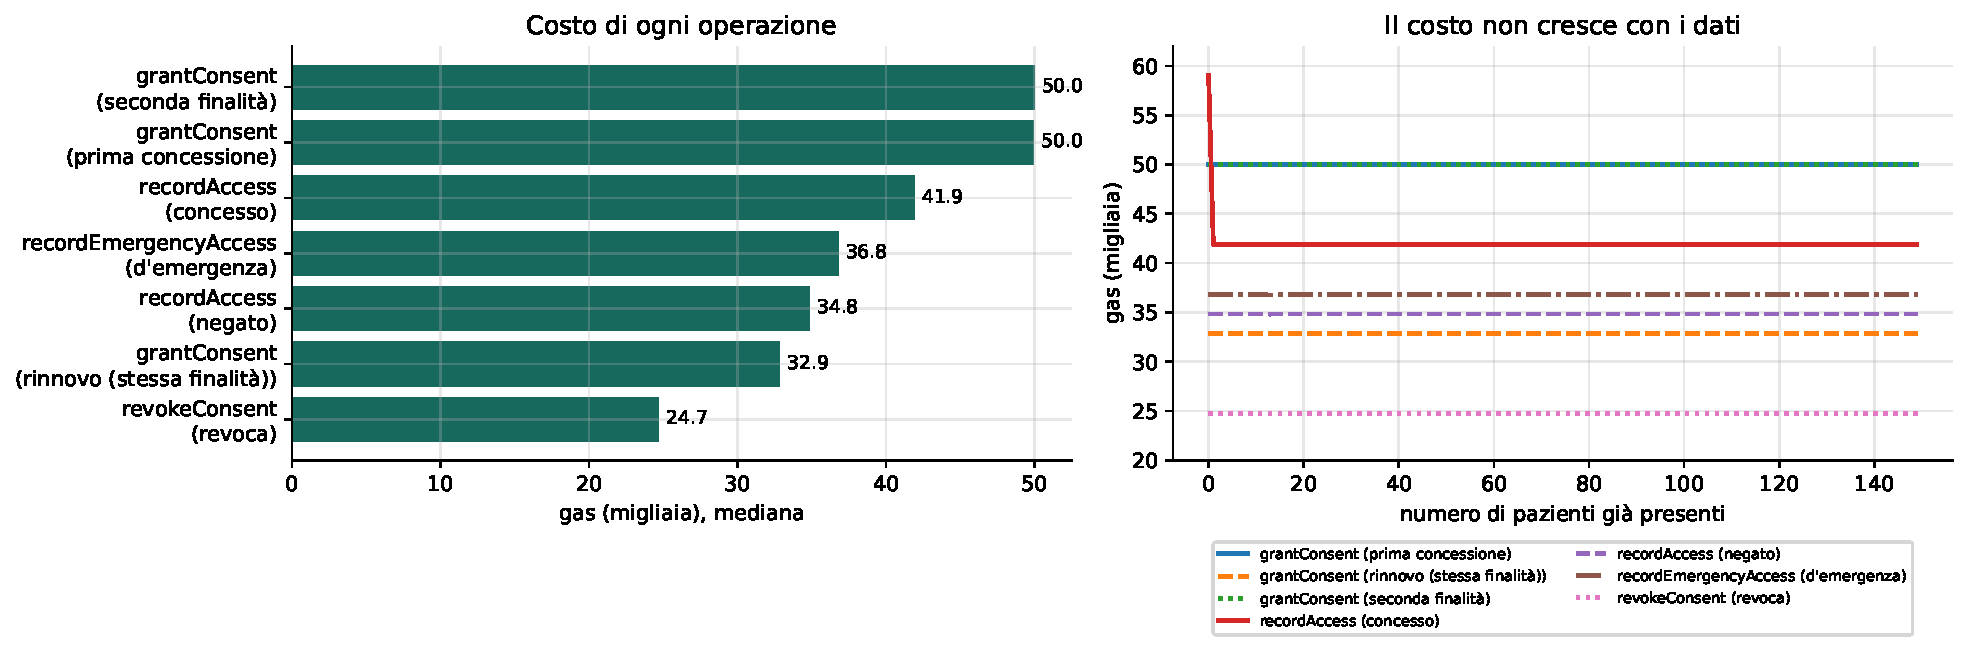
\includegraphics[width=\textwidth]{figure/gas_operazioni.pdf}
\caption{Gas di ogni operazione (a sinistra) e andamento al crescere dei pazienti (a destra).}\label{fig:gas}
\end{figure}

Il costo in euro dipende dal prezzo del gas e dell'ether, che variano di continuo, e dal volume di utilizzo. La figura~\ref{fig:gas-anno} lo calcola in forma parametrica, con ipotesi dichiarate (1 ETH = 3000~€, 50 consensi e 10 revoche al giorno). Con mille accessi al giorno il costo annuo va da qualche migliaio di euro con il gas a 0,1~gwei a quasi un milione con il gas a 20~gwei. È un argomento in più, accanto alla riservatezza dei metadati, a favore di una rete \emph{permissioned} o di secondo livello.

\begin{figure}[H]
\centering
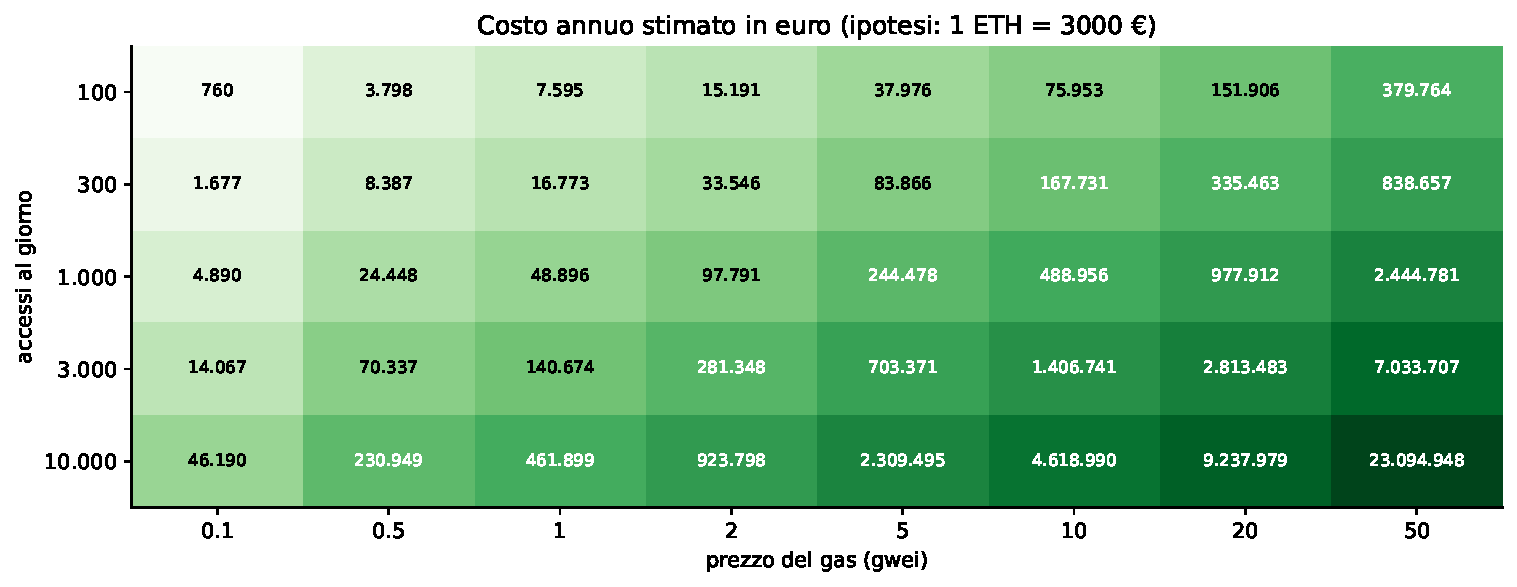
\includegraphics[width=.92\textwidth]{figure/gas_costo_annuo.pdf}
\caption{Costo annuo stimato al variare del prezzo del gas e degli accessi giornalieri (ipotesi dichiarate nel notebook).}\label{fig:gas-anno}
\end{figure}

\subsection{Firme classiche e post-quantistiche}
La figura~\ref{fig:firme} confronta le passkey ES256 e ML-DSA-44 su 300 firme ciascuna. Il prezzo della sicurezza post-quantistica sta quasi tutto nello \textbf{spazio}: la chiave pubblica passa da 77 a 1322 byte, la firma da 71 a 2420, la risposta WebAuthn completa da circa 500 a circa 3600 byte. Il tempo di verifica sul server resta invece dello stesso ordine, circa mezzo millisecondo per entrambi: per un login o per la firma di un referto non è un collo di bottiglia. La dimensione conta di più per i dispositivi con poca memoria e i protocolli con limiti sui messaggi.

\begin{figure}[H]
\centering
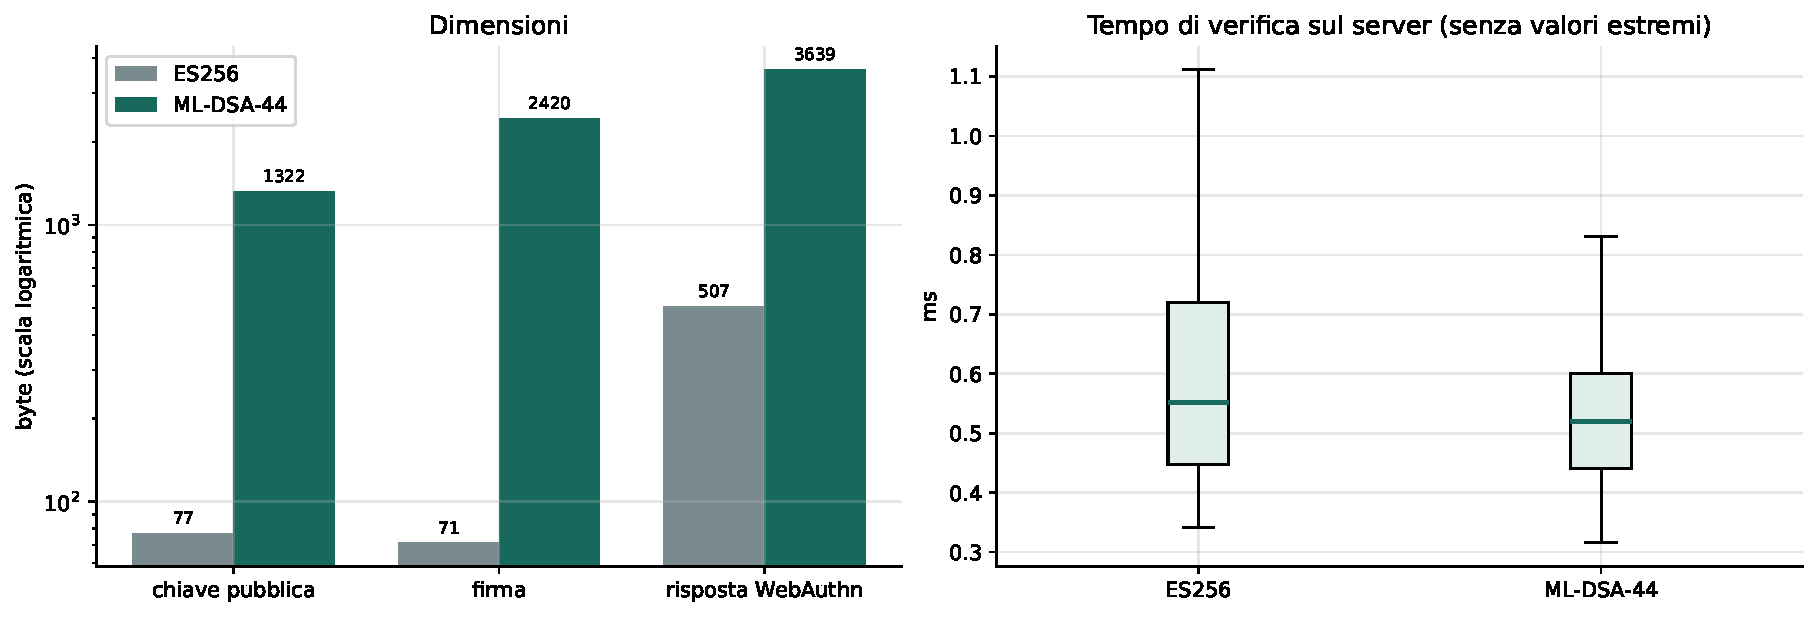
\includegraphics[width=\textwidth]{figure/firme_confronto.pdf}
\caption{Dimensioni (scala logaritmica) e tempo di verifica di ES256 e ML-DSA-44.}\label{fig:firme}
\end{figure}

\subsection{Cifratura ibrida}
Cifrare o decifrare un referto richiede circa 0,15~ms fino a 64~KiB e meno di un millisecondo per un referto di 1~MiB (0,84~ms per la cifratura, 0,56 per la decifratura; figura~\ref{fig:cifratura}). Per i referti piccoli il tempo è dominato dai due meccanismi di incapsulamento, che hanno costo fisso, per quelli grandi da AES-GCM. ML-KEM-768 e X25519 costano decine di microsecondi ciascuno (17 e 24 contro 53 e 33 per incapsulamento e decapsulamento): la componente post-quantistica non pesa sui tempi.

\begin{figure}[H]
\centering
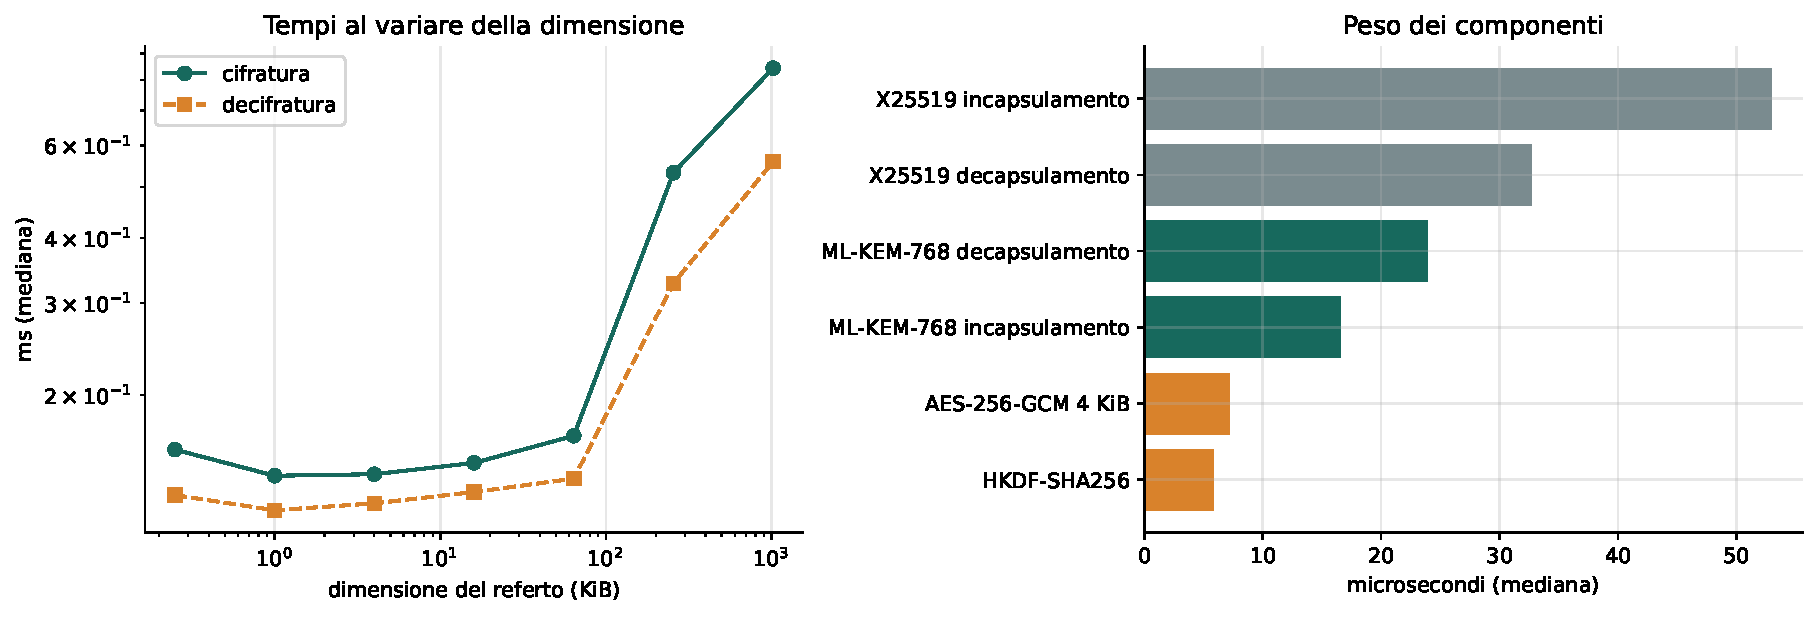
\includegraphics[width=\textwidth]{figure/cifratura_tempi.pdf}
\caption{Tempi di cifratura e decifratura al variare della dimensione del referto e peso dei singoli componenti.}\label{fig:cifratura}
\end{figure}

Per lo spazio (figura~\ref{fig:spazio}) lo schema aggiunge poco meno di 2~KB fissi, soprattutto per il testo cifrato di ML-KEM (1088 byte); i campi sono però salvati come testo base64, che aumenta ogni contenuto di un terzo anche per i referti grandi. Salvarli come dati binari di MongoDB eliminerebbe questo costo.

\begin{figure}[H]
\centering
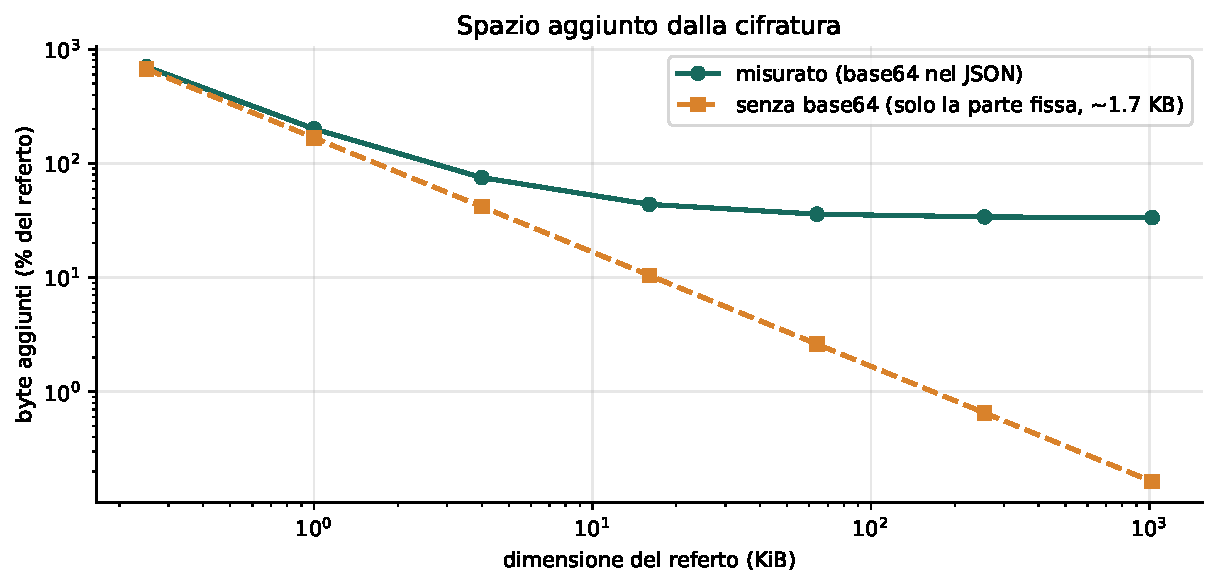
\includegraphics[width=.75\textwidth]{figure/cifratura_spazio.pdf}
\caption{Byte aggiunti dalla cifratura, in percentuale della dimensione del referto: misurati e senza la codifica base64.}\label{fig:spazio}
\end{figure}

\subsection{Custodia delle chiavi}
\paragraph{Argon2id.} Con i parametri del progetto (64~MiB, 3 passate) un tentativo di indovinare la passphrase costa circa 70~ms sulla macchina delle misure (figura~\ref{fig:argon}, a sinistra). A destra il tempo medio di una ricerca esaustiva, al variare della velocità dell'attaccante rispetto a quella macchina: con una passphrase di cinque parole scelte a caso da un dizionario di 7776 (circa 65 bit) servirebbero decine di migliaia di anni anche a un attaccante un milione di volte più veloce, mentre quattro parole (circa 52 bit) scenderebbero a pochi anni. La stima presuppone una passphrase scelta davvero a caso: il controllo sui 12 caratteri minimi non lo garantisce, e una frase nota o prevedibile ha un'entropia molto più bassa.

\begin{figure}[H]
\centering
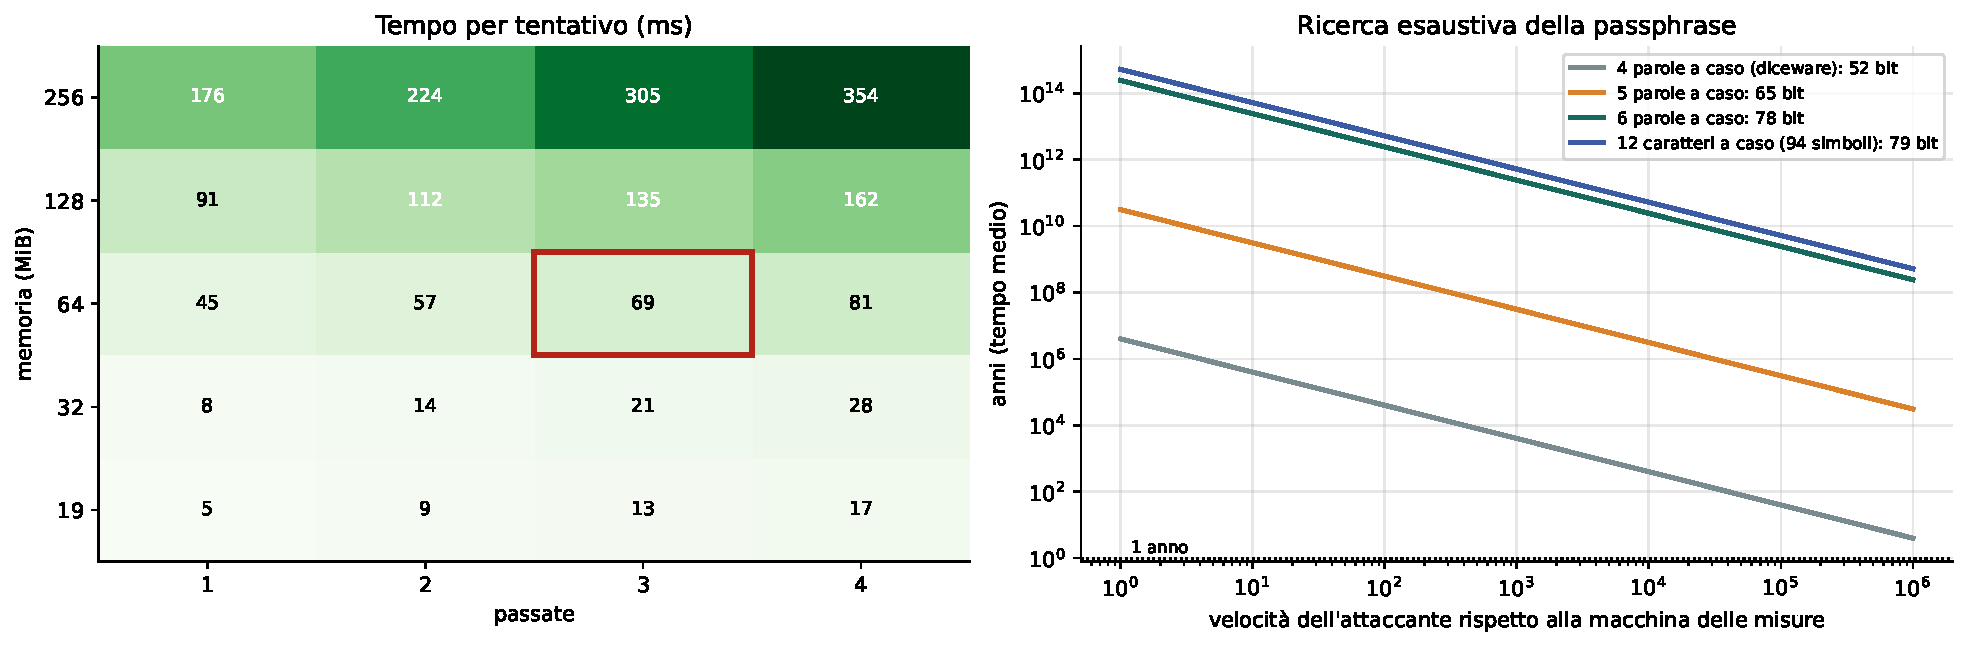
\includegraphics[width=\textwidth]{figure/argon2_costo.pdf}
\caption{Costo di un tentativo al variare dei parametri di Argon2id (in rosso la configurazione del progetto) e tempo medio di una ricerca esaustiva.}\label{fig:argon}
\end{figure}

\paragraph{Schema a soglia.} Per lo schema di Shamir si sono calcolate, con la distribuzione binomiale e una verifica Monte Carlo, la probabilità di perdere le chiavi (meno di $k$ custodi disponibili) e quella che vengano rivelate (almeno $k$ custodi compromessi), assumendo custodi indipendenti. La figura~\ref{fig:shamir} mostra che una copia unica è il caso peggiore su entrambi i fronti, che copie multiple senza soglia riducono la perdita ma moltiplicano il rischio di furto, e che una soglia piena fa il contrario. A destra, con l'ipotesi che ogni custode non sia disponibile nel 10\% dei casi e sia compromesso nel 5\%, il rischio peggiore tra i due è minimo per soglie intorno alla metà del numero di custodi; lo schema adottato, 3 su 5, porta entrambi i rischi sotto l'1\%.

\begin{figure}[H]
\centering
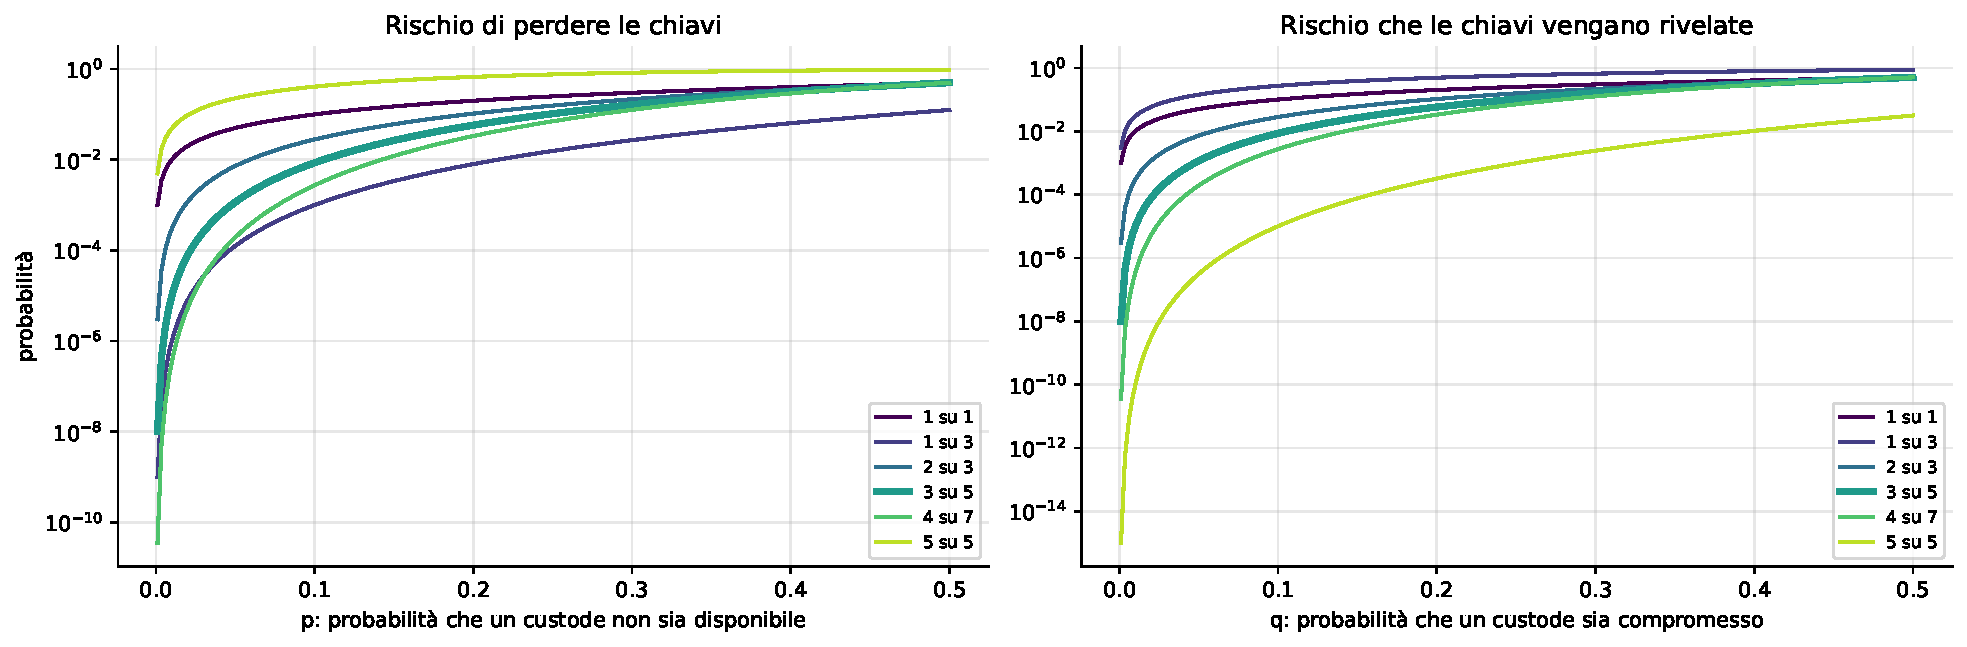
\includegraphics[width=\textwidth]{figure/shamir_rischi.pdf}\\[4pt]
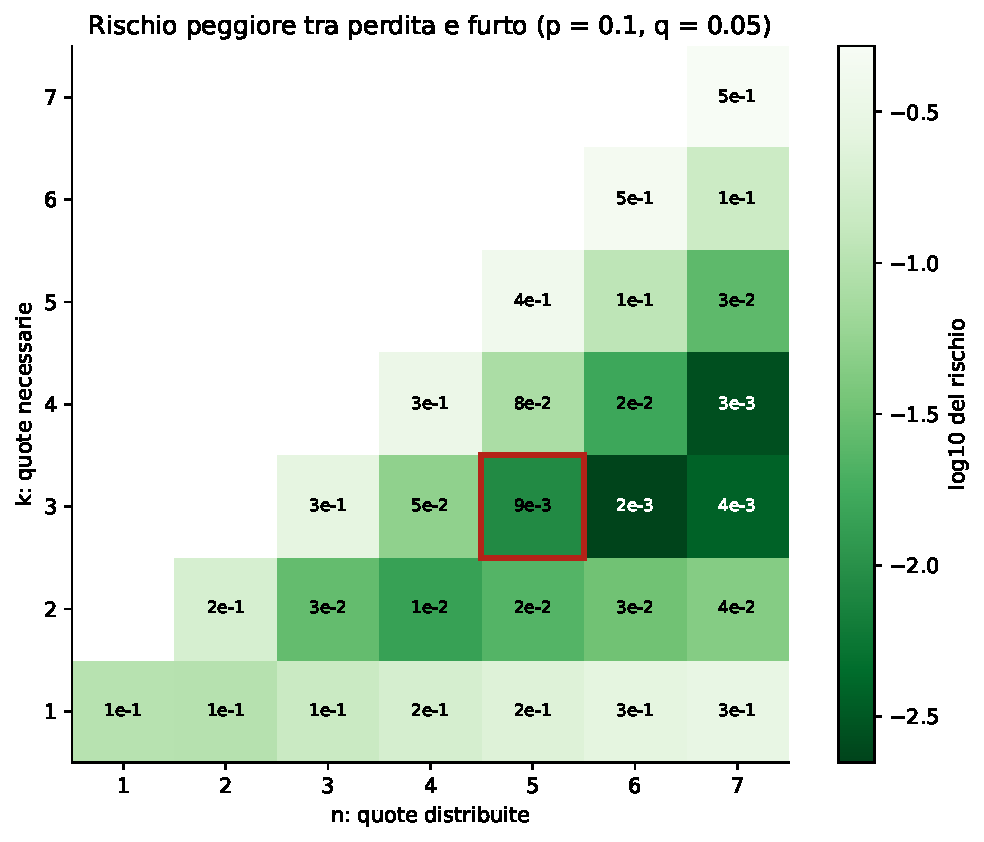
\includegraphics[width=.6\textwidth]{figure/shamir_griglia.pdf}
\caption{Rischio di perdita e di rivelazione delle chiavi per diversi schemi a soglia, e rischio peggiore tra i due per ogni scelta di $k$ e $n$ (in rosso lo schema del progetto).}\label{fig:shamir}
\end{figure}

\subsection{Campagne d'attacco}\label{sec:val-attacchi}
Ogni attacco del modello di minaccia è stato ripetuto 30 volte contro il backend reale, registrando sia l'esito dell'attacco sia quello dell'operazione legittima corrispondente: una difesa che blocca anche gli utenti onesti non è una buona difesa. Per controllare che le prove rilevino davvero i problemi, gli scenari di autenticazione sono stati eseguiti anche sul codice privo delle correzioni della revisione di sicurezza (figura~\ref{fig:attacchi}).

\begin{figure}[H]
\centering
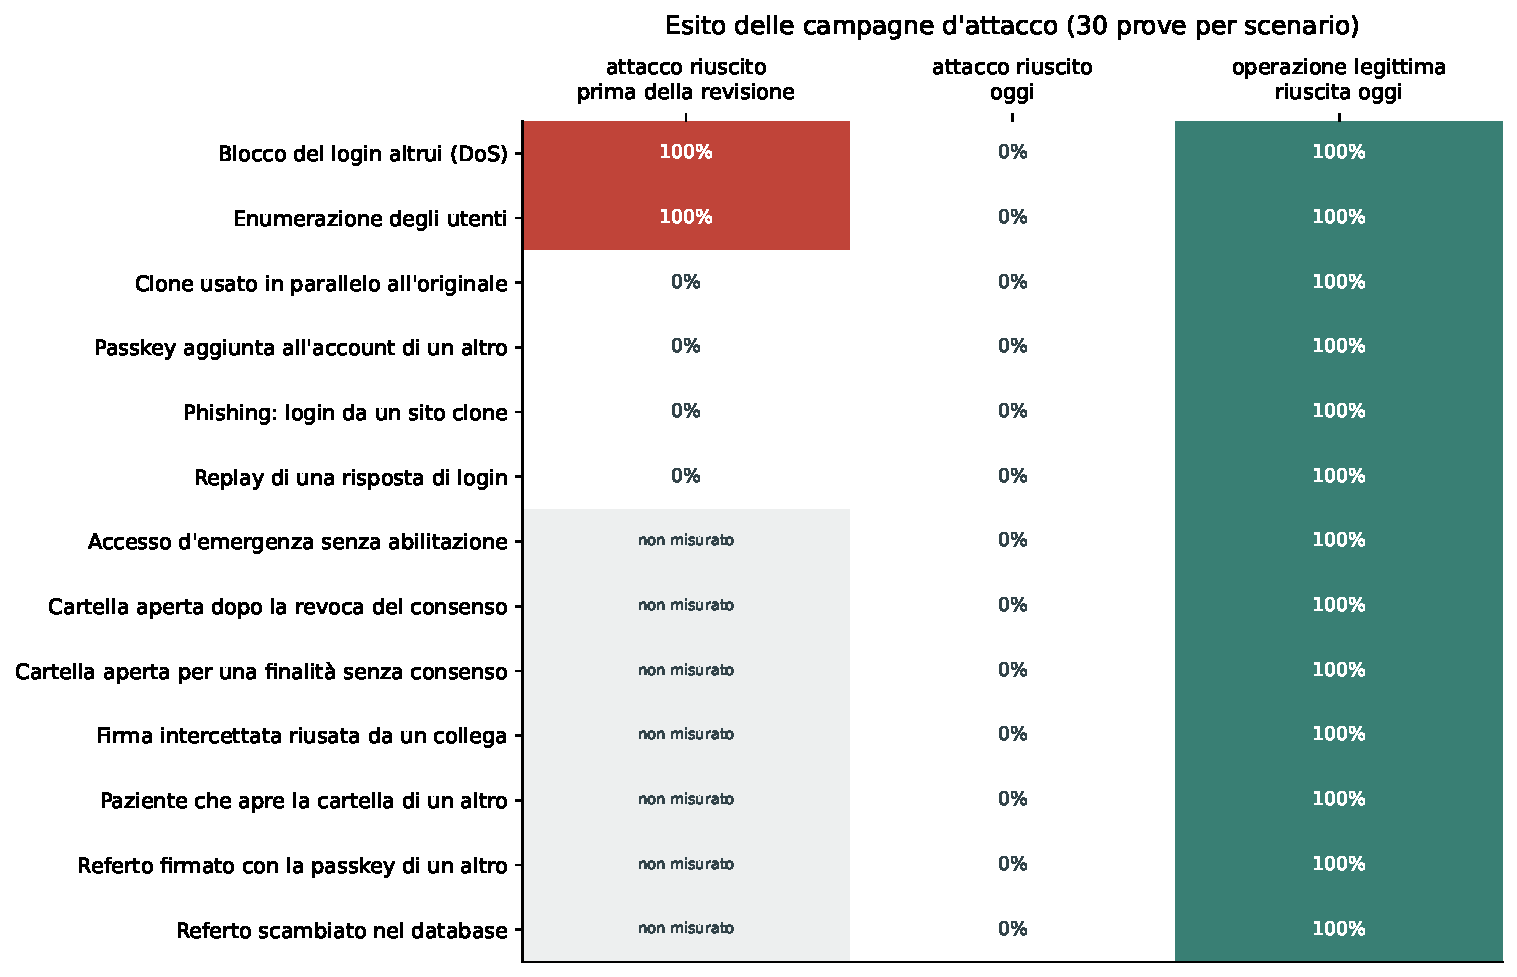
\includegraphics[width=.9\textwidth]{figure/attacchi_matrice.pdf}
\caption{Esito delle campagne d'attacco: percentuale di prove in cui l'attacco o l'operazione legittima sono riusciti.}\label{fig:attacchi}
\end{figure}

Nel prototipo nessun attacco riesce in nessuna prova e tutte le operazioni legittime riescono; senza le correzioni, il blocco del login altrui e l'enumerazione degli utenti riescono nel 100\% delle prove. La figura~\ref{fig:dos} mostra il blocco del login al crescere delle richieste dell'attaccante: senza correzione basta una richiesta al momento giusto, con la correzione la vittima entra sempre.

\begin{figure}[H]
\centering
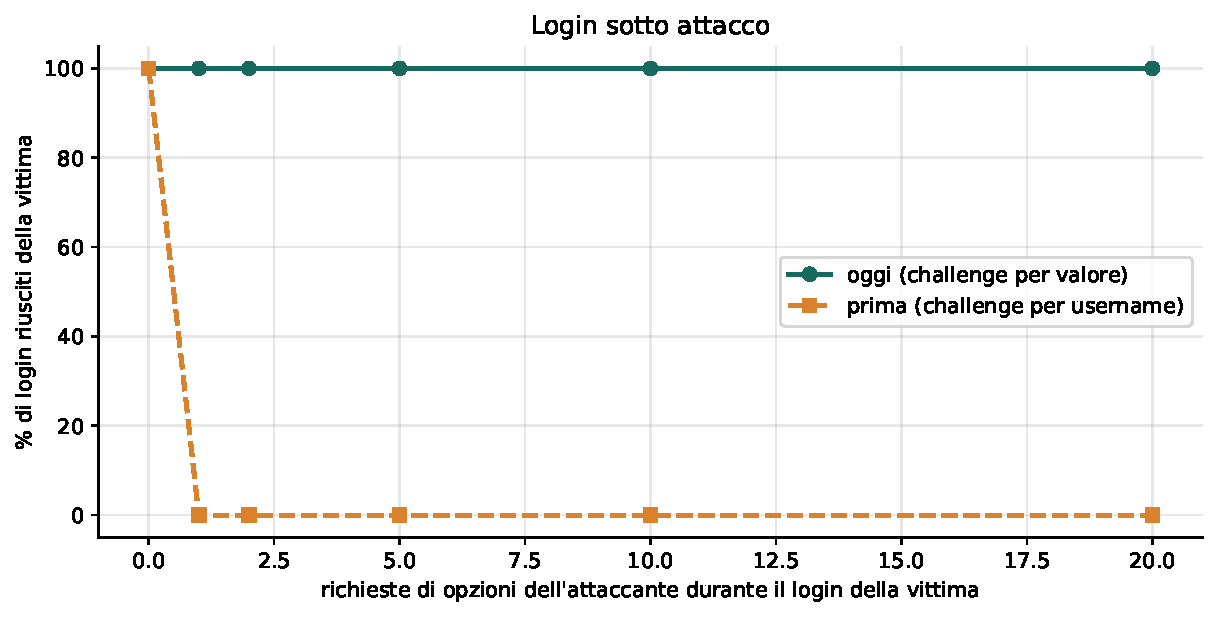
\includegraphics[width=.65\textwidth]{figure/login_dos.pdf}
\caption{Percentuale di login riusciti della vittima al crescere delle richieste dell'attaccante, senza e con la correzione.}\label{fig:dos}
\end{figure}

Zero successi su 30 prove non dimostrano che un attacco sia impossibile, ma che il controllo che lo blocca è sempre attivo, come atteso per controlli deterministici. Le campagne non sostituiscono un penetration test, ma rendono ripetibili le affermazioni di sicurezza della relazione.

\subsection{Limiti della valutazione}
\begin{itemize}
  \item I tempi sono misurati su un solo portatile; quelli della blockchain locale non rappresentano una rete reale, dove la conferma di un blocco richiede secondi, e non sono stati misurati.
  \item Il costo in euro e la stima di forza bruta dipendono da ipotesi esplicite: cambiandole cambiano i numeri, non il metodo.
  \item Il modello di Shamir assume custodi indipendenti; custodi che condividono un luogo o un sistema hanno guasti correlati e un rischio maggiore.
  \item Le campagne d'attacco usano archivi in memoria e una blockchain simulata; le proprietà che dipendono dal database sono coperte dai test d'integrazione su MongoDB.
\end{itemize}

\section{Conclusioni e sviluppi futuri}
% Estensioni possibili: firma dei documenti clinici, credenziali verificabili, TEE.


\printbibliography
\end{document}